%# -*- coding: utf-8-unix -*-
%%==================================================
\chapter{疲劳检测基础知识}

\section{疲劳状态场景}

\subsection{疲劳概述}

疲劳是指人在高强度或者长时间连续工作而产生的一系列不正常的生理和心理变化。目前,心理学上把疲劳分为生理疲劳和心理疲劳两种类型。(1)生
理疲劳,指的是人们在工作活动过程中,由于身体肌肉承担一定的负担而引起的疲劳现象。主要是由体力劳动引起,在临床上主要表现为动作失调、肌肉酸痛等。
(2)心理疲劳,指的是虽然体力上工作强度不大但因工作过程中,脑力活动密集、精神长时间处于高度紧张状态或者工作单调所产生的疲劳现象,也称为精神
疲劳。比如在航空航天领域、长途交通运输领域、核工业领域中,这些工作者往往由于脑力劳动而引起的疲劳,一般认为是心理疲劳。对于精神疲劳,在心理学上,把工作效能降低、工作质量下降和错误率增加作为疲劳的三大客观指标。

世界各国学者经过几十年的精神疲劳研究发现,在精神疲劳时,从检测对象身上采集的生物电信号中,可以提取出与精神疲劳相关的客观量;从检测对象的行为特征中,也可以提取出与精神疲劳相关的表现。其中,生物电信号主要为:(1)可以通过脑电信号中不同的脑电波的变化情况来判定疲劳状态,主要对脑电信号中的$\alpha$波、$\beta$ 波、$\theta$波、$\delta$波进行监测和评估;(2)可以通过对心电信号中的心跳间期进行时域统计分析和和频谱分析,提取出时域和频域中的与疲劳状态相关的变量,从而能够检测到疲劳状态;(3)还可以通过对呼吸的幅度和频率、与交感神经和副交感神经调节相关的生化指标的测量来检测是否处于疲劳状态。行为特征主要为:(1)眼部特征,在疲劳时眨眼频率和眼睛闭合时间都会发生明显的变化,因此,可以通过对眼部特征的提取和对比分析来检测是否处于疲劳状态;(2)视线特征,处于精神疲劳状态时,人们的视线移动速度会明显降低,因此,可以通过对视线的检测来判定疲劳状态;(3)嘴部特征,根据人的行为特征,在疲劳时,往往会经常打哈欠,从而根据嘴部特征能够检测出疲劳状态。

取自\href{https://xueshu.baidu.com/usercenter/paper/show?paperid=1g4g0jv02n7k0eg05g4b08t0tu163338&site=xueshu_se}{基于机器视觉多信息融合的疲劳状态检测}

\subsection{疲劳驾驶场景}
近年来,随着中国经济的飞速发展及汽车制造业技术的成熟,中国的车辆保有量逐年上升,与此同时,我国由于交通事故造成的伤残死亡人数一直是世界上最多的国家之一,每年因交通事故死亡的至少有 50 万以上,交通事故已经被公认为是危害当今人类生命安全的第一大公害。
根据交通事故统计分析表明,交通事故中 80$\% \sim$ 90$\%$是人为因素造成的,驾驶员疲劳驾驶更会使车祸发生的可能性成倍的增加,在我国,大约48$\%$的车祸是由驾驶员疲劳驾驶造成的\footnote{基于级联神经网络疲劳驾驶检测系统设计 \quad \url{https://kns.cnki.net/kcms/detail/11.3092.V.20210305.1723.003.html}}。

所谓的驾驶疲劳, 是指驾驶员由于睡眠不足或长时间持续驾驶而造成的反应能力下降, 其主要表现在驾驶员困倦、打磕睡、驾驶操作失误或完全丧失驾驶能力。交通事故通常就发生在几秒钟的时间内,如果能提前 2 秒钟预警将能减少 92$\%$的交通事故,提前 0.5 秒钟预警,将会避免73$\%$的交通事故,因此,一种高效快速的预警系统,可以拯救成千上万人的生命,避免财产及经济的损失。

疲劳驾驶检测大致可以分为两类:接触法检测和非接触法检测。接触法主要通过可以穿戴的传感器直接获取驾驶人的相关参数指标,由于心率、肌电、皮电、脑电、呼吸频率等参数能有效的反映驾驶人的生理状况,因此通过可穿戴式传感器直接提取驾驶人的相关参数指标即可判断驾驶人的疲劳状况。通过该方法开展研究较为成熟,检测结果有效可靠, 准确率高, 但是由于传感器直接穿戴在身体上,容易影响驾驶人的正常驾驶。非接触法主要是通过车辆行驶状态进行检测及基于视觉的驾驶人检测。车辆行驶状态进行检测是通过检测机动车的方向盘转角、方向盘转向力、行驶轨迹、车辆的速度等参数来间接判别驾驶人的疲劳状况。由于车辆行驶状态受到驾驶人的驾驶习惯、道路环境状况等诸多因素的影响,因此,该检测方法的可靠性和准确率不高。

由于驾驶人的疲劳状态会反映到面部特征上,如频繁的眨眼、打哈欠、点头等,因此可以通过检测这些特征指标进行疲劳判断,很多学者开展该方面的研究(参考这两篇论文《\href{https://xueshu.baidu.com/usercenter/paper/show?paperid=671cbaaddd0c5e8365feebf7cc1145ad&site=xueshu_se&hitarticle=1}{基于面部行为分析的驾驶员疲劳检测方法}》,《\href{https://xueshu.baidu.com/usercenter/paper/show?paperid=1p5k08u0hf5y04b07v1s0gx0nu129126&site=xueshu_se&hitarticle=1}{基于多尺度池化卷积神经网络的疲劳检测方法研究}》)。 史瑞鹏等在《\href{https://xueshu.baidu.com/usercenter/paper/show?paperid=126t08102r3x0r002v760pj018696892&site=xueshu_se&hitarticle=1}{一种基于卷积神经网络的疲劳驾驶检测方法}》一文中提出了一种基于MTCNN 算法的疲劳驾驶检测方法,实现了疲劳驾驶的检测判定。戴诗琪等在《\href{https://xueshu.baidu.com/usercenter/paper/show?paperid=cd41c261d06bee71082a1f570326e23e&site=xueshu_se}{基于深度学习的疲劳驾驶检测算法}》一文中先用 HOG 算子进行人脸检测和人脸对齐,之后通过深度卷积神经网络实现了驾驶员的眼部疲劳特征的提取。F Zhang等在《\href{https://xueshu.baidu.com/usercenter/paper/show?paperid=b02b21c4b90a17cbe1ee9bb2004d0b6f&site=xueshu_se&hitarticle=1}{Driver Fatigue Detection Based on Eye State Recognition}》一文中利用红外视频对戴眼镜时的眼睛状态进行了疲劳检测,识别精度较高。

取自\href{https://kns.cnki.net/kcms/detail/61.1114.th.20201228.1452.013.html}{融合面部特征的机动车驾驶人疲劳检测}

\subsection{疲劳施工场景}

建筑施工行业一直被认为是高危行业。随着生产力的进步,各类施工机械(特别是大型机械)在建筑工程中的应用越来越普遍。工程机械的应用,在提高建筑业生产效率的同时,也带来了诸多安全问题。根据住建部安全事故情况通报,大量工程安全事故源于施工机械的安全问题。

在《\href{https://kns.cnki.net/kcms/detail/11.5823.tu.20210201.1703.039.html}{基于计算机视觉技术的施工机械操作员疲劳作业检测方法}》一文中,作者构建了一种基于计算机视觉技术的施工机械操作员疲劳作业检测方法。采用 dlib 模型标注 68 个人脸特征点,计算实时的眼纵横比(EAR)和嘴纵横比(MAR)值,并取前 30 秒视频作为样本计算出相应的阈值,进而计算出眨眼频率、平均眨眼时长、眼睑闭合时间百分比(PERCLOS)以及哈欠频率这四个指标值,利用归一化方法进行指标融合,依据综合疲劳指标的取值和持续时间采取不同的疲劳应对措施。结果表明本论文提出的综合疲劳指标能够反映不同情境下检测对象疲劳状态的变化趋势,其眨眼状态判定的正确率在 $95\%$ 左右。
...(再找一个例子)

\subsection{疲劳听课场景}

在学校课堂上,部分学生由于沉重的学业压力,课堂效率不高,甚至在课堂上出现昏昏欲睡的现象。目前,对于上课疲劳的学生多数是依靠老师提醒或者同学提醒来提高注意力,但这两种方式都收效甚微。疲劳状态使学生的课堂效率低下,从而学习成绩下降,甚至产生了对学习的厌恶感,而为了提高成绩,他们在将利用更多的课余时间,花费更多的精力。这样恶性循环,对他们的身心健康也产生了巨大的负面影响。当前多数的研究仅仅只是针对疲劳的危害,而对于真正如何解决上课疲劳的方法还不明确。

在《\href{https://xueshu.baidu.com/usercenter/paper/show?paperid=1q1y04j09m4y0xu0we0c0mf0fk289643&site=xueshu_se}{基于图像处理的上课疲劳检测}》一文中,作者采用中值滤波,直方图均衡化等传统图像处理方法来检测学生疲劳状态。

在《\href{https://xueshu.baidu.com/usercenter/paper/show?paperid=190t08j0my790eb0rr7c0g90xf140982&site=xueshu_se}{基于深度学习的学生课堂疲劳状态的分析与研究}》一文中,作者结合深度学习当中的卷积神经网络训练出的网络模型,提高了对脸部特征检测的准确率,并且在目前PERCLOS疲劳判断的基础上引入新的变量,将嘴部的张合状态是否过大作为判断疲劳的另一指标.通过在课堂上对学生的眼部,嘴部等区域进行采样与分析,结合更新后的疲劳判断指标与方法进而给出疲劳与否的判断。

在2006年《\href{https://arxiv.org/ftp/arxiv/papers/1803/1803.07952.pdf}{An Exercise Fatifue
Detection Model Based on Machine Learning Methods}》一文中,作者对体育活动导致的人体疲劳进行了研究。作者将实时获取的临床数据作为输入参数,诊断方法包括时间序列分析、频响分析、去趋势振荡分析、近似熵和标准熵分析。实验结果表明,疲劳检测精度为98.65$\%$。

\section{疲劳检测数据类型及对应特征}

\subsection{主观评定量表}

主观评定法是通过填写量表来对脑力疲劳情况进行评定,例如卡罗琳斯卡嗜睡量表(Karolinska Sleepiness Scale, KSS)和斯坦福嗜睡量表(Stanford Sleepiness Scale, SSS),该种方法具有一定的可信度 ,同时又具有很强的主观性,容易受多种因素影响。

KSS将主观疲劳划分成9个等级:(参考《\href{https://xueshu.baidu.com/usercenter/paper/show?paperid=8dc58cb15e4230afae7bb495ec0b83a1&site=xueshu_se}{Subjective and objective sleepiness in the active individual}》)
\begin{enumerate}
	\item 极度警觉
	\item 非常警觉
	\item 警觉
    \item 一般警觉
    \item 不太警觉但也无困意
    \item 有一些困意倾向
    \item 有困意,但是不需要太多努力保持清醒
    \item 有困意,且需要一定的努力保持清醒
    \item 非常困倦,需要极大的努力保持清醒 \\
\end{enumerate}

SSS将主观疲劳划分成7个等级:(参考《\href{https://xueshu.baidu.com/usercenter/paper/show?paperid=85150b8651495a78e9e8344dd4c0302a&site=xueshu_se&hitarticle=1}{Validation of the Karolinska sleepiness scale against performance and EEG variables - ScienceDirect}》)

\begin{enumerate}
	\item 感觉有活力、生机、警觉、清醒
	\item 处于高水平的功能状态,但非顶峰状态,能够集中注意力
	\item 松弛、清醒、没有处于完全的警觉状态、有响应
    \item 有点模糊、不处于顶峰状态、松懈
    \item 模糊,开始丧失保持清醒的兴趣、行为缓慢
    \item 嗜睡,喜欢躺下,抗拒睡眠,糊涂
    \item 总在幻想、快速入睡、放弃保持清醒
\end{enumerate}


\subsection{生物电信号}

\subsubsection{心电信号}

1)ECG 和 PPG

常见的心电信号包括:心电图(ECG)和光容积描记术(PPG),这两类信号常常用于疲劳检测的准确估计方法之中,但是由于它们需要通过在身体上嵌入心电信号传感器来采集数据,使得它们在疲劳驾驶检测中具有局限性。然而,由于非侵入式传感器领域的进展,电流传感器可以嵌入方向盘或座椅皮带,缓解了侵入式传感器在疲劳检测种带来的不便。

最初,非侵入式心电图传感器被嵌入到驾驶员座椅或者腰带中,然而,由于材质的原因,这两种方法都容易因为材质厚度而产生误差。为了克服这一问题,Jung 在《\href{https://xueshu.baidu.com/usercenter/paper/show?paperid=bd19bce061c995470f2f5df1beef2481&site=xueshu_se&hitarticle=1}{Driver fatigue and drowsiness monitoring system with embedded electrocardiogram sensor on steering wheel}》一文中提出将电极嵌入到方向盘。

从心电信号中我们可以提取出两个重要的用于疲劳检测的参数:心率(HR)和心率变异性(HRV),而疲劳检测的视觉指标包括:打哈欠和深呼吸。两名受试者参与了真实环境的测试,最后研究表明,HRV随着疲劳而增加。这种方法(电极嵌入方向盘)展现了很好的结果,但是需要高精度的传感器来观察驾驶员状态从正常到疲劳的微小变化。其次,就是驾驶员的手必须安放在在方向盘上。

相对于ECG,PPG也可以用来估计驾驶员的疲劳程度。Li and Chung在《\href{https://xueshu.baidu.com/usercenter/paper/show?paperid=ff6ce7a5353e5830f88f2ef24de4a947&site=xueshu_se}{Detection of driver drowsiness using wavelet analysis of heart rate variability and a support vector machine classifier,}》一文中提出了一种基于PPG传感器的驾驶疲劳检测的方法,其中PPG 传感器放置在方向盘上。作者从PPG信号中提取出HRV 特征,并用SVM进行训练,完成对驾驶员疲劳状态的分类。其中数据集的真实标签采用的是PERCLOS指标的分析结果,以及KSS调查问卷的结果。在他们的研究中,四名志愿者(三名男性和一名女性)参与了实验,最后实验表明该方法具有$95\%$ 的疲劳检测精度。即使这种方法是非侵入性的,它也容易受到人为操作的错误。

翻译于\href{https://xueshu.baidu.com/usercenter/paper/show?paperid=1r7a06p0ve7m08y0s32w0jq04r498130&site=xueshu_se}{Driver Fatigue Detection Systems: A Review}

2)PPG原理

在医疗领域,通常使用心电描记术(Electrocardiography,ECG)测量生理电信号来实现心率和心脏活动的检测。ECG信号虽然精准并且信息丰富,但是由于测量ECG信号常常要在身体多个部位连接传感器电极,在临床医疗领域外并没有得到太多的应用。现在各种可穿戴设备采用的都是光电容积脉搏波描记法(photoplethysmographic,PPG)来简单测量心率。

采用PPG原理的光学心率传感器往往有一个发光元件,测量心率时LED光射向皮肤,透过皮肤组织反射回的光被光敏传感器接收并转换成电信号再经过AD转换成数字信号,整个过程可简化为:光 $\dashrightarrow$ 电 $\dashrightarrow$ 数字信号。其测量原理为:当光照透过皮肤组织然后再反射到光敏传感器时,光照会发生一定的衰减。像肌肉、骨骼、静脉和其他连接组织等对光的吸收是基本不变的(前提是测量部位没有大幅度的运动),但是血液不同,由于动脉里有血液的流动,那么对光的吸收自然也有所变化。当我们把光转换成电信号时,正是由于动脉对光的吸收有变化而其他组织对光的吸收基本不变,得到的信号就可以分为直流DC信号和交流AC信号。提取其中的AC信号,就能反应出血液流动的特点。

心率估计和监测对于确定一个人的生理和心理状态非常重要,传统的测量心率的方法都是接触式的,如电极式心电图(ECG),通过电极片感应人体的心动电流来测量心率;在可穿戴设备如智能手表上,最常用的是利用光电容积脉搏波(PPG)来进行测量,但同样需要紧密接触皮肤。接触式的测量方式虽然较为准确,但必然会带来很多不适与不便,尤其在某些特殊的场景下,无法使用接触式的测量方式,因此后来出现了rPPG光电容积脉搏波描记术\footnote{基于视频分析的rPPG心率检测综述 \quad \url{https://zhuanlan.zhihu.com/p/83674059}}。\\

3)rPPG的出现

2008年,Verkruysse等人首先研究证明,通过摄像头采集人的面部视频,可以从中分析出和心率相关的光电容积脉搏波描记信号,从而实现远程测量心率,相关原理被称为远程光电容积描记术(Remote Photoplethysmography (rPPG)) 。rPPG与传统的PPG 原理是一样的,每次心跳带来的血液流动会在人体皮肤组织的微血管中形成周期性的变化,从而对吸收或反射光也会有一个周期性的信号,如图\href{table:2-15}{2-15}所示。这个周期性的信号人眼无法观测到,但是可以通过高清摄像头采集到的人脸数据中分析出来,从而检测心率,所以这种方法也被称为超感知的心率检测。rPPG的优越性不仅体现在它的检测对象不需要佩戴任何传感器,所以可用于新生儿、烧伤患者、或是长时间的病房监护,甚至可以用于家用的老年人长时生理监测或是司机开车时的疲劳状态监测等,而且因为普通的高清摄像头便宜方便,使用简单且分布广泛,也让rPPG有了很大的应用前景。ECG,PPG,rPPG 三者之间的比较如表\href{table:2-1}{2-1}}所示。

但这种基于视频分析的远程心率检测受环境和检测对象的影响比较大,为了提高其检测的准确度和鲁棒性,研究者们分别从环境光照以及检测对象的运动状态两个方向上进行了大量的研究。最近,一些研究也开始将二者同时进行考虑。但总的来说,在使用场景和检测鲁棒性上,基于视频分析的远程心率检测还有很大的应用场景和研究空间。\\

\begin{figure}[!htp]

\centering
%\begin{minipage}[t]{5in}
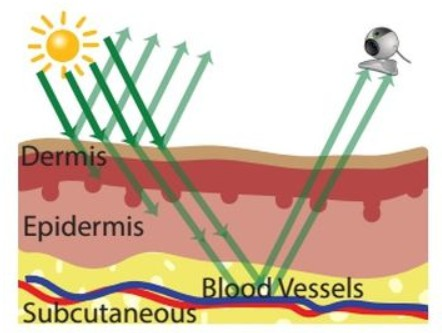
\includegraphics[width=3.5in]{example/PPG.jpg}
\caption{rPPG原理}
\label{fig:1-2}
%\end{minipage}

\end{figure}

4)BVP信号

血容量脉冲(BVP)信号是一种由心脏周期性地收缩和扩张,导致脸部血容量周期性地变化所形成的微弱的生理信号,与其他生理信号相比,它可由普通光学摄像头拍摄人脸彩色视频获取,无需与人体接触。研究表明,BVP信号中包含有心率值和呼吸频率值[\cite{osman2015supervised},\cite{poh2010advancements},\cite{monkaresi2013machine}], 当人紧张或害怕时,由于血液不能及时流到动脉末梢,BVP 信号幅度偏低,而当人处于放松状态时,随着血液流至末梢,BVP信号幅度增加。



\begin{table}[]
\centering
\caption{ECG,PPG,rPPG三者优缺点比较}
\resizebox{\textwidth}{!}{%
\begin{tabular}{|l|l|l|l|l|}
\hline
信号                                                            & 仪器          & 提取的特征 & 优势     & 存在问题       \\ \hline
ECG(心电描记术) &
  \begin{tabular}[c]{@{}l@{}}传感器电极(身体多\\ 个部位)\end{tabular} &
  心率 &
  精准,信息丰富 &
  \begin{tabular}[c]{@{}l@{}}应用面窄,在临床医疗领域\\ 外很少应用\end{tabular} \\ \hline
\begin{tabular}[c]{@{}l@{}}PGG(光电容积脉\\ 搏波描记法)\end{tabular} &
  \begin{tabular}[c]{@{}l@{}}智能手表等可穿戴设备(光学\\ 心率传感器)\end{tabular} &
  心率 &
  准确 &
  接触式,应用面窄 \\ \hline
\begin{tabular}[c]{@{}l@{}}rPPG(远程光电容积\\ 脉搏波描记法)\end{tabular} & 摄像头(获取面部视频) & 心率    & 测量方式简单 & 准确性、鲁棒性待研究 \\ \hline
\end{tabular}%
}
\end{table}

\subsubsection{脑电信号}

脑电图是测量大脑活动的黄金标准,它作为疲劳的良好指标,可以根据不同频段信号的特性,反映清醒和睡眠之间的过渡。脑电图可以通过连接在头皮上的扁平电极来提取。

在频域上,脑电信号可分为5个频段,如图\href{fig:1-1}{1-1} 所示。图中有$\gamma$波(30-42 Hz),$\beta$波(13-30 Hz), $\alpha$波(8-13 Hz), $\theta$波(4-8 Hz) 和$\delta$ 波(0.5-4 Hz)。 当一个人处于警觉状态时,比如在执行认知任务时,$\beta$波就会出现,而有时也可能在睡眠早期出现。$\theta$波与睡眠早期有关,深度睡眠以$\delta$ 波表现。$\alpha$波在放松状态下出现,表现出疲劳迹象。

\begin{figure}[!htp]

\centering
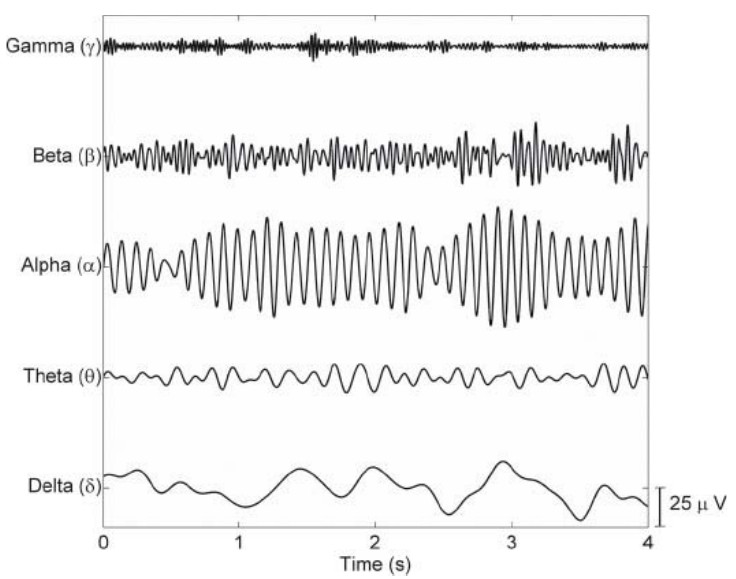
\includegraphics[width=3.5in]{example/eeg.jpg}
\caption{EEG信号}
\label{fig:1-1}

\end{figure}

Borghini等在《\href{https://xueshu.baidu.com/usercenter/paper/show?paperid=0847723933c31c989a8acc86884b0e17&site=xueshu_se}{Assessment of mental fatigue during car driving by using high resolution eeg activity and neurophysiologic indices}》一文中引入了基于$\alpha$纺锤波(峰值)的EEG疲劳指数,在真实驾驶环境中提取被试者的脑电图。结果表明,随着疲劳的增加,脑电图$\alpha$ 纺锤波增加。尽管结果较为不错,但实验中并没有提到参与者的数量,因此用户的准确性受到了影响。最近的一项研究《\href{https://xueshu.baidu.com/usercenter/paper/show?paperid=ec185cd8a8353f4bf65b7057235907c4&site=xueshu_se}{Driver Fatigue Classification With Independent Component by Entropy Rate Bound Minimization Analysis in an EEG-Based System}》则建议使用三层前馈贝叶斯神经网络结构进行数据分类(无论是疲劳的还是非疲劳的),特征在输入分类器之前通过ICA-ERBM 进行分离,再采用自回归(AR)模型对数据进行分割并提取特征。该文在模拟环境中提取了43名受试者的脑电信号,并通过视觉疲劳迹象、眼电信号、车道偏差和问卷调查对结果进行了验证。该方法的疲劳检测精度达到$89.7\%$。

翻译于\href{https://xueshu.baidu.com/usercenter/paper/show?paperid=1r7a06p0ve7m08y0s32w0jq04r498130&site=xueshu_se}{Driver Fatigue Detection Systems: A Review}

\subsubsection{肌电信号}

肌电信号(EMG)传感器通过电极记录肌肉细胞产生的电势,而表面肌电信号(sEMG)是测量皮肤表面肌肉产生电势的一种手段。从sEMG中提取的时域和频域特征可以用来预测肌肉疲劳,并利用均值和中值频率的变化、电激活和均方根(RMS)振幅等特征进行疲劳检测。在《\href{https://xueshu.baidu.com/usercenter/paper/show?paperid=243e90cdbefb97cf245f038386f0da1a&site=xueshu_se&hitarticle=1}{EMG-based analysis of change in muscle activity during simulated driving}》一文中,作者使用15-30 Hz频段的信号功率进行肌肉疲劳检测。在模拟环境中,通过将sEMG电极放置在驾驶员颈部、背部、肩膀和手腕上,从驾驶员身上提取sEMG。11个人参与了这项研究,最终得出的结论是15-30 Hz 频带的功率随着疲劳而增加。sEMG传感器需要很强的嵌入性,因此在驾驶员疲劳实时检测中适用性有限。

翻译于\href{https://xueshu.baidu.com/usercenter/paper/show?paperid=1r7a06p0ve7m08y0s32w0jq04r498130&site=xueshu_se}{Driver Fatigue Detection Systems: A Review}

\subsubsection{眼电信号}

EoG是测量位于眼睛前后的角膜和视网膜电位差的一种方法,EoG 通过连接在眼睛左右两侧的电极来测量眼睛的运动。对于EoG 数据,可以采用基于能量分布的熵值对其进行分类。在《\href{https://xueshu.baidu.com/usercenter/paper/show?paperid=8c21b4420996c3c1d4b4584356cdd59a&site=xueshu_se&hitarticle=1}{EOG-based drowsiness detection using convolutional neural networks,}》 一文中,22名受试者参与实验。作者从参与者眼睛周围精确放置的电极中提取EoG,接着通过CNN从EoG中提取特征,最终实验分析得出的结论是:疲劳响应误差随着疲劳增加而增加(疲劳程度越高,预测误差越大?)。

由于电极放置在眼睛附近,可能会对司机造成干扰。Zhang等提出了一种将电极放置在驾驶员前额上的EoG测量技术,其结果还是比较不错的,然而,基于EoG 传感器的方法在实时驾驶疲劳检测中应用还是很有限。

\subsubsection{多种生物电信号融合}

如果融合多种生物电信号,模型可以获得更好的性能,疲劳估计也会更准确。Sun和Yu在《\href{https://xueshu.baidu.com/usercenter/paper/show?paperid=43e8f07b1c090997f279272a41f920c9&site=xueshu_se&hitarticle=1}{An innovative nonintrusive driver assistance
system for vital signal monitoring}》一文中,利用衣服上非侵入性电极采集受试着的ECG、利用帽子上的电极采集EEG, 利用挂在车顶上的电极采集EoG,如图\href{fig:1-2}{1-2} 所示,其中30个人(8名女性和22名男性)参与了这项实验。使用Wierwille 和Ellsworth标准(基于疲劳的视觉线索)作为评价疲劳的ground truth,记录眼睑活动、EEG和HRV来估计疲劳。据推断,闭眼时间和眼睛闪烁频率随疲劳增加而增加;$\alpha$波和$\beta$波功率密度随疲劳降低而降低;LF/HF 和SDNN随疲劳降低而降低;RMSSD、低频和高频随疲劳增加而增加。在《\href{https://xueshu.baidu.com/usercenter/paper/show?paperid=72e4bf79735d66cef42a2f56c6bdb211&site=xueshu_se&hitarticle=1}{Automated Detection of Driver Fatigue Based on Entropy and Complexity Measures}》研究中,作者也建议使用多种生物电信号进行驾驶疲劳检测。

\begin{figure}[!htp]

\centering
%\begin{minipage}[t]{5in}
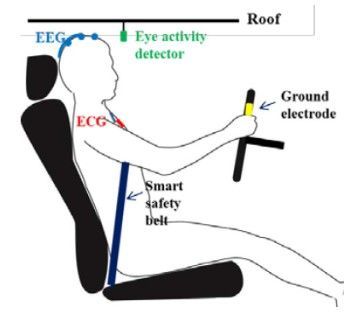
\includegraphics[width=2in]{example/multi_biological.jpg}
\caption{EEG,ECG,EoG数据采集}
\label{fig:1-2}
%\end{minipage}

\end{figure}

基于生物电信号的疲劳检测技术如表\href{table:1-1}{1-1}所示。生物电信号特征是疲劳检测的直接衡量指标,但由于传感器的侵入性,其在驾驶员疲劳实时检测中应用受到限制。

\begin{table}[!htp]

\centering
%\begin{minipage}[t]{5in}
\caption{生物电信号汇总}
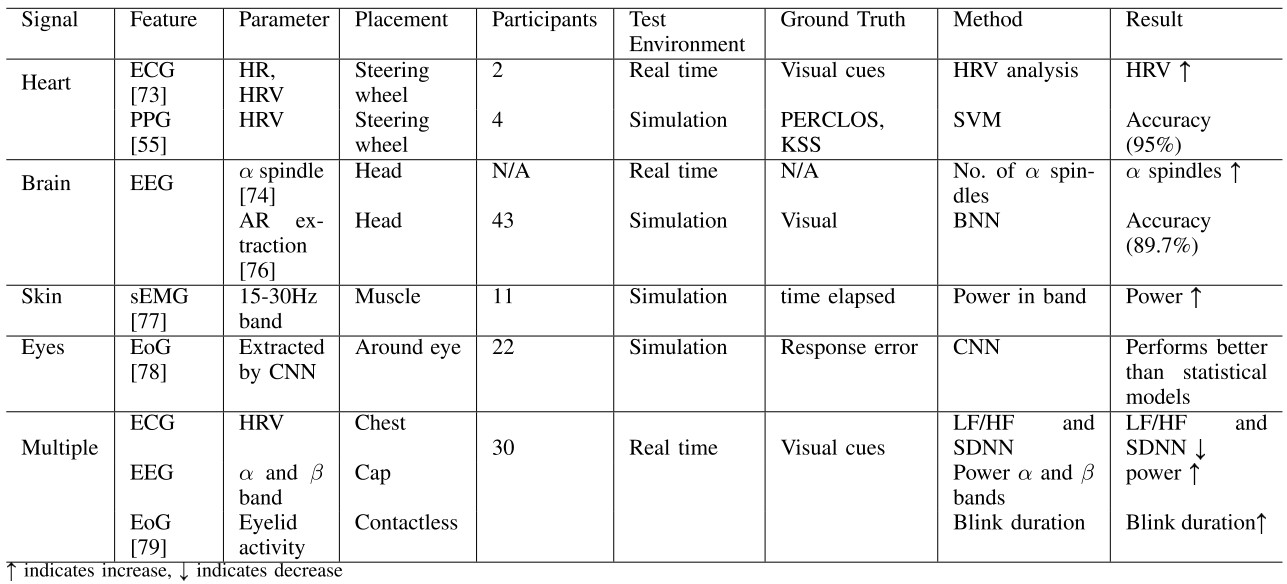
\includegraphics[width=6in]{example/biological.jpg}
\label{table:1-1}
%\end{minipage}

\end{table}

\subsection{行为特征}

驾驶员面部特征和头部的运动可以用来检测疲劳。行为特征包括眨眼频率、闭眼时间、闭眼时间百分比(PERCLOS)、姿势、凝视方向和点头的频率。基于行为特征的疲劳检测系统大致可以归类为基于眼睛、嘴,脸和头的疲劳检测系统。

\subsubsection{眼睛特征}

研究发现,闭眼频率、眼睑距离、睁眼频率等特征可以作为疲劳检测的指标。在《\href{https://xueshu.baidu.com/usercenter/paper/show?paperid=42c02572346008a3b76421d3d2e499a5&site=xueshu_se&hitarticle=1}{A driver face monitoring system for fatigue and distraction detection}》一文中,模糊系统将疲劳程度分为低、正常和高三种水平,利用Haar-like特征检测器对图像中的人脸进行检测,利用模板匹配和水平投影对人脸图像进行特征提取。该方法在实际驾驶环境中对五个人进行了测试,并以客观评价为依据(比如使用Wierwille 和Ellsworth标准的基于疲劳的视觉线索),对疲劳特征进行分类。该人脸跟踪方法精度不高,计算复杂,且在低光照条件下精度大大降低。

在2017年的《\href{https://xueshu.baidu.com/usercenter/paper/show?paperid=2e0968b70318946da955342ec643266a&site=xueshu_se}{Towards Detection of Bus Driver Fatigue Based on Robust Visual Analysis of Eye State}》一文中,疲劳检测系统是专门为公交车司机设计的,该方法利用安装在公交车上的圆顶摄像头来监控司机的驾驶行为。使用睁眼次数和PERCLOS作为疲劳检测的特征,使用梯度直方图(HoG)检测头部和肩部,使用支持向量机检测驾驶员,而人脸检测和眼睛检测分别由OpenCV人脸检测器和眼睛检测器来完成,对于眼睛的开度,使用线性和光谱回归来计算。该技术已在23名驾驶员的真实驾驶环境中进行了测试。由于该疲劳实验是自模拟的,因此不加入ground truth方法。然而该技术一开始是为公交车设计的,需要在车上安装圆顶摄像机,因此并不适用于所有的车辆。

\subsubsection{嘴巴特征}

眼睛活动检测是一种常见的疲劳检测方法,然而,打哈欠和张口程度也可以作为疲劳检测的指标。在《
\href{https://xueshu.baidu.com/usercenter/paper/show?paperid=fd12f51013020b4d8efeeb3666104ff6&site=xueshu_se}{Driver's Fatigue Detection Based on Yawning Extraction}》 一文中,通过打哈欠识别来检测驾驶员是否疲劳。使用支持向量机来检测视频帧中的人脸,利用梯度边缘检测器定位嘴部。此外,使用霍夫圆变换检测嘴巴是否处于打哈欠状态。通过设计一个哈欠计数器,根据哈欠个数来检测司机的疲劳程度。该技术已经在真实环境中进行了测试,但是疲劳是由参与者自行模拟的,参与者的数量也没有提到。该系统具有98$\%$的精度,但需要包括更多的功能来检测疲劳。

\subsubsection{面部特征}

相对于预先定义特征,我们可以通过深度学习模型来提取特征,在《
\href{https://xueshu.baidu.com/usercenter/paper/show?paperid=a9b574549a36e94db6af2b728361eee9&site=xueshu_se&hitarticle=1}{Drowsy driver detection using representation learning}》一文中,特征选择是通过CNN得到的,并将特征用于视觉的疲劳检测。在CNN最后一层中使用softmax分类器对所选特征进行分类,归类为疲劳和不疲劳。在实验中,30个具有不同特征,肤色,毛色和疲劳程度的受试者参与了模拟研究。该系统的准确度达到92.33 $\%$。在他们实验中,从面部图像序列中提取了500个融合了Gabor变换的特征向量。在一天不同时间,不同光照水平和不同机位下采集驾驶员的行车视频。为了从面部图像中挖掘疲劳模式,使用了频繁模式挖掘算法,即使此方法具有99.2 $\%$的高检测精度,但该技术仅在单个参与者上进行了测试,因此需要进一步在多个参与者上测试,这样才会更准确地描述该方法在系统中的真实准确性。

\subsubsection{多行为特征融合}

为了提高精度,我们可以同时使用多个行为特征进行疲劳检测。Bergasa等在《\href{https://xueshu.baidu.com/usercenter/paper/show?paperid=878001d7c60796581b6cfcecaf6c59e5&site=xueshu_se}{Real-time system for monitoring driver vigilance}》一文中,利用眼睛,面部和头部特征,将PERCLOS,闭眼持续时间,眨眼频率,点头频率,面部位置和凝视方向输入到模糊推理系统(FIS)中进行疲劳检测。十名参与者在实际驾驶场景中参与了实验,实验分析得出的结论是:该系统在晚上运行良好,然而在白天,尤其是在晴天的时候,系统的性能会下降,并且该系统不太适合于戴眼镜的驾驶员。由于该方法在光照变化条件下适用性有限,因此需要进一步的改进。表
\href{table:1-2}{1-2} 总结了基于行为特征的疲劳检测方法。

\begin{table}[!htp]

\centering
%\begin{minipage}[t]{5in}
\caption{行为特征汇总}
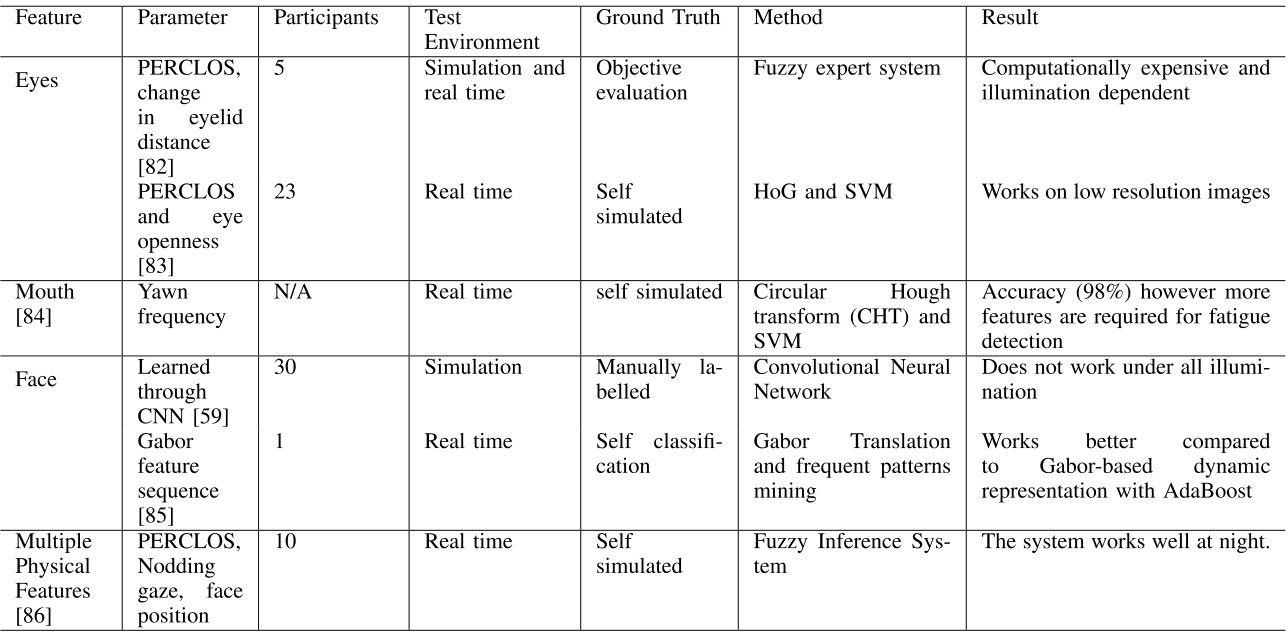
\includegraphics[width=6in]{example/physical.jpg}
\label{table:1-2}
%\end{minipage}

\end{table}

\subsection{车辆特征}

交叉车道和方向盘转角等特征的偏差是检测疲劳驾驶的指标。而异常活动,如刹车和加速器的压力变化,驾驶员座位上的负载分布和车速,也是检测疲劳驾驶的重要指标。其中车辆特征可分为方向盘转角、车道偏差和驾驶员的姿势变化。

\subsubsection{方向盘转角}

将方向盘转角作为特征,是识别驾驶员是否疲劳的常用方法,McDonald等在
《\href{https://xueshu.baidu.com/usercenter/paper/show?paperid=3cf717214e2143abd5449c89f8cfd8d1&site=xueshu_se}{Real-time detection of drowsiness related lane departures using steering wheel angle}》一文中,利用方向盘转角和随机森林算法检测车道偏离情况。与PERCLOS相比,该方法更准确,可以提前6 秒预测与疲劳相关的车道偏离。该算法在爱荷华大学国家高级驾驶模拟器的数据集上进行了测试,72名参与者参与了这项研究。研究人员使用修正的观察者嗜睡评分(mORD) 量表,从原始模拟数据中提取与嗜睡相关的车道偏离。每分钟读取一次,直到车道偏离。作者使用眼睛检测软件-FaceLab,定位追踪视频中的人眼,并从中提取PERCLOS特征。随机森林是由一系列随机选择特征的决策树来训练的。这项研究并没有忽视PERCLOS作为一种疲劳检测指标的重要性,然而该文作者要强调的是,在疲劳检测方面,方向盘转角(Steering Wheel Angle)也是一种较好的指标。

在《\href{https://xueshu.baidu.com/usercenter/paper/show?paperid=520e8ddf646e97a09f78d361e1a76151&site=xueshu_se&hitarticle=1}{Online detection of driver fatigue using steering wheel angles for real driving conditions}》一文中,作者提出了一种基于SWA的方法,根据方向盘转角计算近似熵(ApEn)。作者还计算了自适应分段线性近似(APLA),用来估计疲劳状态的相似度。这次驾驶考试是在从北京到秦皇岛的高速公路上进行的,因为高速公路上乏味的驾驶环境,更容易让司机感觉到疲劳。该方法的精度为78.01$\%$,需要进一步提高才能应用于疲劳检测。

\subsubsection{司机姿势}

疲劳会直接影响驾驶员的驾驶姿势,而驾驶姿势的变化可以通过负荷中心位置(LCP)来检测。LCP可以通过座椅上的压力传感器来测量,在《\href{https://xueshu.baidu.com/usercenter/paper/show?paperid=b2bc2c266ebbbf17c1b5f6837af20612&site=xueshu_se&hitarticle=1}{Estimation of Driver Fatigue by Pressure Distribution on Seat in Long Term Driving}》一文中车身压力传感器安装在车辆的驾驶员座椅上,人们发现,在开始时,压力分布在整个座椅上,然而久而久之压力开始集中在座椅靠背的一个点上。实验中每20分钟读取一次压力读数,持续15分钟,但该方法只在一个参与者身上测试过。

\subsubsection{车道偏离}

除SWA外,车道偏差也被广泛应用于驾驶员的疲劳检测。在2009年《\href{https://xueshu.baidu.com/usercenter/paper/show?paperid=d275df140848b004c3b9deb6c9f9f365&site=xueshu_se}{Detection of driver fatigue caused by sleep deprivation}》 一文中,Yang等人设计了一个模拟驾驶环境的试验台,有12名参与者参与,其中对睡眠的剥夺程度是实验中唯一的独立变量。作者给出了4 个刺激响应任务:1)当出现变道标志时变道行驶(APVT) 2) 当出现变换两车道标志时,变换两车道行驶(VPVT) 3)听到铃声后,按下绿色按钮(SLCT) 4) 当看到屏幕上出现红色提示物时,按下绿色按钮(DLCT)。作者发现,APVT、VPVT、SLCT和DLCT的均值和标准差与参与者睡眠时间有一定相关度。该方法仅在模拟器上测试过,并没有在实际路况上进一步测试。

\subsubsection{多种车辆特征融合}

为了提高疲劳检测的准确性,我们可以利用多个车辆特征对驾驶员进行疲劳检测。Wakita等人在2006年《\href{https://xueshu.baidu.com/usercenter/paper/show?paperid=545e342c13b390e67fa55f6f79a851e4&site=xueshu_se}{Driver Identification Using Driving Behavior Signals}》 一文中,利用车辆速度、制动踏板、加速踏板和车前距离等特征来估计驾驶员疲劳情况。作者将这些特征输入到高斯混合模型(GMM) 和海利模型中,对比研究表明,高斯模型比海利模型效果更好,该方法在模拟器上的精度为81$\%$,在真实车辆上检测精度为73$\%$。

表\href{table:1-3}{1-3}对车辆特征进行总结。


\begin{table}[!htp]

\centering
%\begin{minipage}[t]{5in}
\caption{车辆特征汇总}
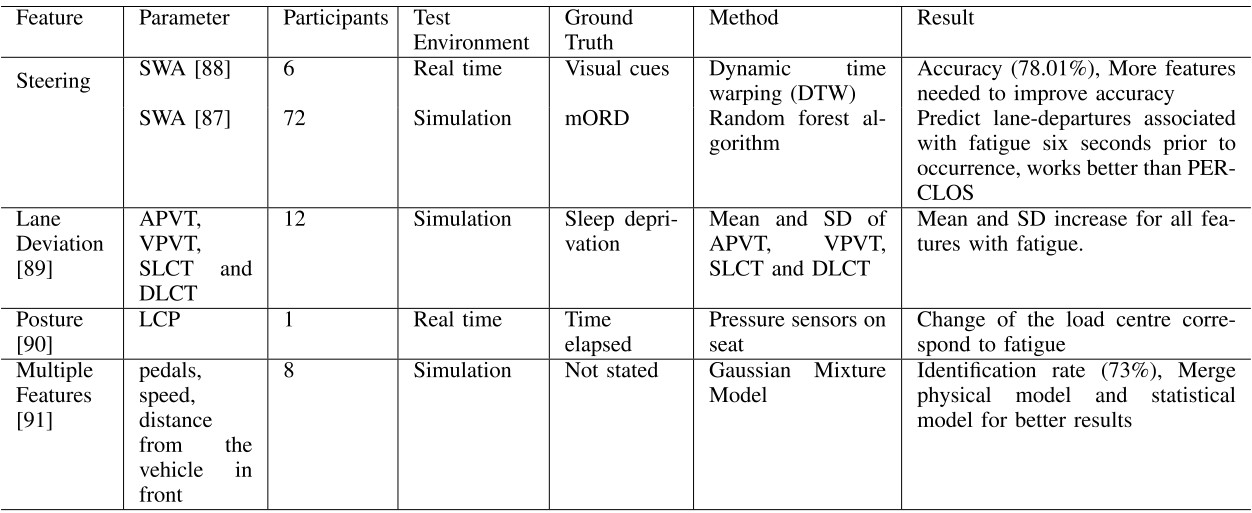
\includegraphics[width=6in]{example/vehicular.jpg}
\label{table:1-3}
%\end{minipage}

\end{table}

\subsection{语音特征}

对于疲劳检测,常见的语音特征包括:MFC系数(mel-spectral coefficients),发音速度、反应速度和发音准确度。但是需要注意以下某些特殊情况:通常说话者可以在相当活跃的状态下进行缓慢的交流,说话者可能存在言语缺陷等,这些都会对基于语音特征的疲劳预测准确度带来干扰。

在2006年《\href{https://xueshu.baidu.com/usercenter/paper/show?paperid=7e674fe5eb722228c0d9e0bcc5188b55&site=xueshu_se}{Detecting Fatigue From Voice Using Speech Recognition}》论文中,作者提出利用语音识别,通过计算MFC系数来预测疲劳水平。这项工作主要研究该相关系数是否会因说话人疲劳水平不同而发生变化。系数分配给特定的音素,并在睡眠开始潜伏期中对系数进行测试。作者指出,与之前的研究相比,准确率提高了20$\%$。

在2015年《\href{https://xueshu.baidu.com/usercenter/paper/show?paperid=3c1f7acf94bff8e975cf6838f7e53a74&site=xueshu_se&hitarticle=1}{Fatigue Detection Using Voice Analysis}》论文中,有人提出通过对语音的分析来确定说话人的疲劳程度。该研究者利用MatLab和PRAAT 仪器对语音进行提取,研究强度、传输频率、共振峰、吞吐量、声频、语音持续时间、期望值、均方差、标准差、能量、功率、语音质量、MFC系数、均值自动校正、语音间隙持续时间等参数在语音中的影响。该文采用神经网络、支持向量机、K-means 分类器、naïve 贝叶斯分类器和logistic回归对计算得到的数据进行进一步分类,其中支持向量机(SVM)结果为98.9$\%$。

\subsubsection{MFCC}

感知实验表明,人耳对于声音信号的感知聚焦于某一特定频率区域内,而非在整个频谱包络中。耳蜗的滤波作用是在对数频率尺度进行的,在1000Hz以下为线性,在1000Hz以上为对数,这就使得人耳对低频比高频更敏感\footnote{梅尔倒谱系数特征(Mel-frequency cepstral coefficients,MFCC) - \url{https://www.cnblogs.com/ytxwzqin/p/10717978.html}}。 心理物理学研究表明,人类对语音信号频率内容的感知遵循一种主观上定义的非线性尺度,该非线性标度可被称为“Mel”标度。

一般来说,声音的频率和人耳所听到的声音高低不成正比,而是与音调(人们为了描述声音高低而定义的概念)成正比,声音的频率分布与临界频带分布相一致。梅尔频率标度的单位是 Mel,它是为了描绘音调而被定义出来的,它更生动地反映出了频率和音调的非线性关系。

梅尔倒谱系数特征(Mel-frequency cepstral coefficients,MFCC)是将人耳的听觉感知特性和语音产生机制相结合,因此目前大多数语音识别系统广泛使用这种特征。对频率轴不均匀划分是MFCC特征区别于前面普通倒谱特征的最重要的特点,变换到Mel域后,Mel带通滤波器组的中心频率是按照Mel刻度均匀排列的。

语音的MFCC特征是基于人耳感知实验得到,将人耳当成特定的滤波器,只考虑某些特定频率成分。这些滤波器是在频域上不均匀分布的。更多的滤波器聚集于低频部分,高频部分的滤波器较少。采样率16Khz时,如图\href{figure:2-9}{2-9}实例所示:

\begin{figure}[!htp]

\centering
%\begin{minipage}[t]{5in}
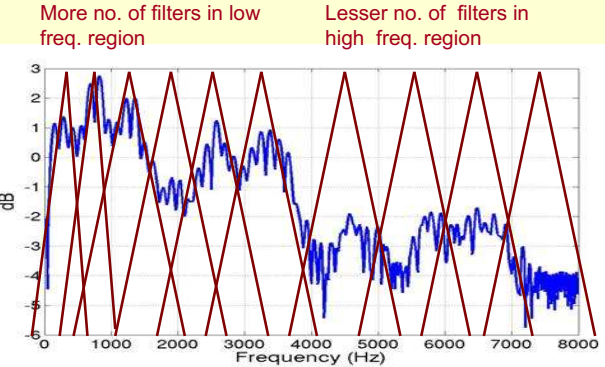
\includegraphics[width=4.5in]{example/MFCC.png}
\caption{Mel滤波器模拟人耳感知实验}
\label{table:2-9}
%\end{minipage}

\end{figure}

MFCC是一种倒谱特征,计算意义见图\href{figure:2-10}{2-10}:

\begin{figure}[!htp]

\centering
%\begin{minipage}[t]{5in}
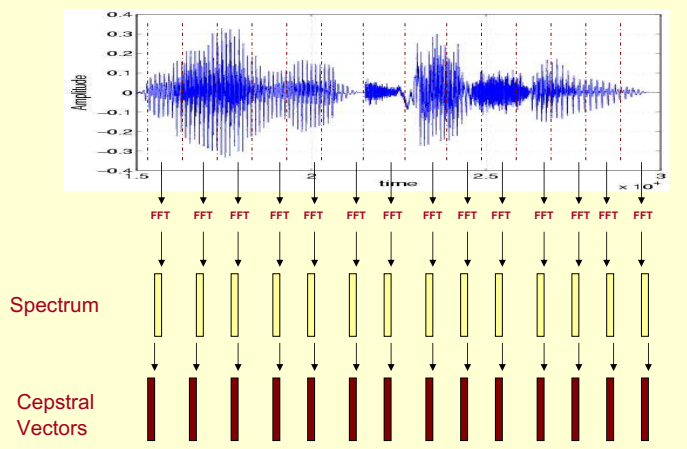
\includegraphics[width=4.5in]{example/MFCC1.png}
\caption{MFCC计算及其意义}
\label{table:2-10}
%\end{minipage}

\end{figure}

其中,对于声音信号,一般会进行分帧后再提取特征,利用不同的窗函数实现。

MFCC可以描述为:Spectrum $\rightarrow$ Mel-Filters $\rightarrow$ Mel-Spectrum。先计算当前帧数据的频谱(通过FFT)得到短时谱,再经过mel滤波器滤波,输出对数MEL能量谱,经过DCT(Discrete cosine transform)去相关,得到MFCC系数(此时特征维数由DCT系数数目决定)。

mel三角带通滤波器有两个主要目的:对频谱进行平滑化,并消除谐波的作用,突显原先语音的共振峰。因此对于一段语音的音调或音高,是不会呈现在 MFCC 参数内,换句话说,以 MFCC 为特征的语音辨识系统,并不会受到输入语音的音调不同而有所影响。此外,还可以降低运算量。

经过特征提取,语音信号可以通过一系列的倒谱向量表示。可参考图\href{figure:2-11}{2-11}:

\begin{figure}[!htp]

\centering
%\begin{minipage}[t]{5in}
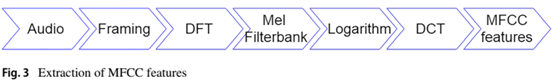
\includegraphics[width=4.5in]{example/MFCC2.png}
\caption{MFCC计算及其意义}
\label{table:2-11}
%\end{minipage}

\end{figure}

\subsection{不同疲劳检测特征的比较}

研究表明,许多疲劳检测相关的特征都取决于受试者嗜睡的程度,而嗜睡的程度又进一步取决于一天中某个时间点、司机驾车的时长以及司机距离上一次睡眠的时长。当开发一个疲劳检测系统时,我们要考虑到采集数据的传感器不应干扰或阻碍驾驶员行车,并且检测过程是自主实时进行的。

主观调查报告KSS 可以对疲劳进行合理地检测和分类,但它要求驾驶员经常报告自己的状态,一方面干扰了驾驶员行车,另一方面可能导致驾驶员报告错误,因为在2009年《\href{https://www.baidu.com/link?url=e2XCc1kghhdalxqr4l4AHikYS8UUH347GgQY7ceGatW3wzN3R_YQqLv5FKa-in3kLRGY85EmQNFesRAKR7mN9_&wd=&eqid=b9e2839900227c2d00000002603e3b1c}{Drivers’ misjudgement of vigilance state during
prolonged monotonous daytime driving}》一文中,研究发现当驾驶活动达到3 小时后,驾驶员对自身健康状况的有效判断能力会明显下降,因此主观报告对于驾驶员疲劳检测的适用性有限。

从生物电信号中提取出来的特征可以得到可靠和准确的结果,因为它们代表人体真实的内部状态;然而,为了获取诸如脑电图、心电图和表面肌电信号等数据,需要将多个电极连接到受试者身体上。与人体相连的电极使得疲劳检测具有侵入性,这不利于对驾驶员疲劳的实时检测。另一个影响因素可能是:通过众多电极获取的脑电图信号对外部因素产生的噪声非常敏感(参考2006年的《\href{https://xueshu.baidu.com/usercenter/paper/show?paperid=01fdcb2a2c4b5c05b4170b9c0d553a32&site=xueshu_se&hitarticle=1}{A complex analysis of the driver behavior from simulated
driving focused on fatigue detection classification}》)。此外,EoG信号是通过放置在眼睛附近的电极来获取的,这可能会阻碍司机的驾驶。在前面提到的所有生物电信号特征中,心电图可以通过一种侵入性较小的方法进行测量;然而,在同种环境下,心电的表现因个体多样性而存在差异,因此可以用于人类识别(参考2005年的《\href{https://xueshu.baidu.com/usercenter/paper/show?paperid=f241adbfa836f474cc236e9b7e9b110a&site=xueshu_se}{ECG to identify individuals}》,2010年的《\href{https://xueshu.baidu.com/usercenter/paper/show?paperid=b2174f5b8f08112d8247be00de45f5e0&site=xueshu_se&hitarticle=1}{Identification of individuals using electrocardiogram}》)。

生物传感器既复杂又昂贵,采集的信号需要通过大量的预处理才能避免噪音,而且在信号采集过程中容易受到驾驶员的影响,对于实时的驾驶员疲劳检测,行为特征和车辆特征更可取,因为它们都不是侵入性的。由于驾驶员的疲劳状态会直接影响对车辆的控制或车辆的偏离的程度,因此车辆特征也可以用于疲劳检测。然而,正如《\href{https://xueshu.baidu.com/usercenter/paper/show?paperid=56d31fd90628e2f1207568df728e0c81&site=xueshu_se}{Subjective sleepiness, simulated driving performance and blink duration: Examining individual differences}》所说的,疲劳对每个个体基于车辆特征的影响并不总是相似的。同样,与眨眼频率相比,侧卧位的标准差也存在显著的个体差异,车辆特征容易受到个人驾驶习惯、天气和交通状况的影响。在城市交通场景中,转向和车道偏差会变得不稳定,即使没有开始疲劳,标准差也会增加。因此,在上面介绍的三种疲劳检测特征中,行为特征可以认为是疲劳检测中最有效特征。

2009年,Barr 等人在《\href{https://xueshu.baidu.com/usercenter/paper/show?paperid=aded0de3ebb58d07e23230c62153fce6&site=xueshu_se}{An evaluation of emerging driver fatigue detection measures and technologies}》研究中发现,光照对疲劳检测的可靠性和准确性有相当大的影响。作为行为特征的PERCLOS,是使用最广泛的疲劳检测技术之一,然而它没有考虑到个体差异的影响。基于驾驶员行为特征的方法依赖于图像处理,因此,它需要在所有室外条件下,如白天、夜晚、雨天、晴天和阴天具有鲁棒性。为了尽量减少室外环境的影响,研究人员安装了红外摄像机,由于红眼效应,红外摄像机使瞳孔的检测更容易,然而,红外摄像机不会在所有照明条件下检测到明亮的瞳孔。

2017年,De Naurois等在《\href{https://xueshu.baidu.com/usercenter/paper/show?paperid=76bb81fc6b65675fa178861a1109e741&site=xueshu_se&hitarticle=1}{Detection and prediction of driver drowsiness using artificial neural network models}》一文中对基于生物电信号、驾驶员行为和车辆特征的疲劳检测进行了对比分析。利用心率、眼睛状态、头部位置、方向盘、车道偏差、踏板力、车速等特征检测驾驶员疲劳。在检测过程中,作者将生物电信号、驾驶员行为和车辆特征输入到神经网络进行训练。此外,人工神经网络也使用额外的参数进行训练,如驾驶时间和参与者信息等。

在某些情况下。将驾驶员行为特征、驾驶时间和参与者信息结合起来,可以得到最佳的疲劳检测结果。由于近十年来非接触式心率测量领域的发展,远程测量PPG (rPPG) 成为可能。RPPG是从人脸颜色变化中提取出来的,可以通过普通的RGB相机采集得到,这使得它很容易与行为特征一起集成训练,用于驾驶疲劳检测。目前,利用rPPG 进行驾驶员疲劳检测的研究相对较少。

根据Horne和Reyner在1995年《\href{https://xueshu.baidu.com/usercenter/paper/show?paperid=3848bbb16ac092c9224bd450fb80436c&site=xueshu_se}{Sleep related vehicle accidents}》一文中的研究,驾驶员的年龄和驾驶时间在睡眠相关事故中起重要作用,因此,外在原因也可以归因于疲劳。在2007年的《\href{https://xueshu.baidu.com/usercenter/paper/show?paperid=ab695119186c9f9bdd1a9144ca287d43&site=xueshu_se}{Advanced driver fatigue research}》一文中,作者发现其他因素如道路限速和环境因素也可以作为驾驶员安全与否的考虑因素。在本研究中,作者发现:对于疲劳检测,单一的特征不能做到可靠性的疲劳估计,因此多种特征组合才能得到准确的预测结果;相比于其他特征,EEG,ECG在实时疲劳检测中并不是很实用;车辆特征依赖于其他一些因素,如天气、驾驶风格和交通状况,在城市环境中可能无法提供可靠的结果;然而,车辆特征可以用于在高速公路上行驶的长途司机的疲劳检测。

结果表明,驾驶员的行为特征最适合作为疲劳检测的特征。为了提高与行为特征的融合效果,建议利用一天的某个时间点、司机驾驶时间和rPPG信号进行特征的融合。表\href{table:1-4}{1-4} 对三种疲劳检测特征的比较进行了总结

\begin{table}[!htp]

\centering
%\begin{minipage}[t]{5in}
\caption{三种疲劳检测特征的比较}
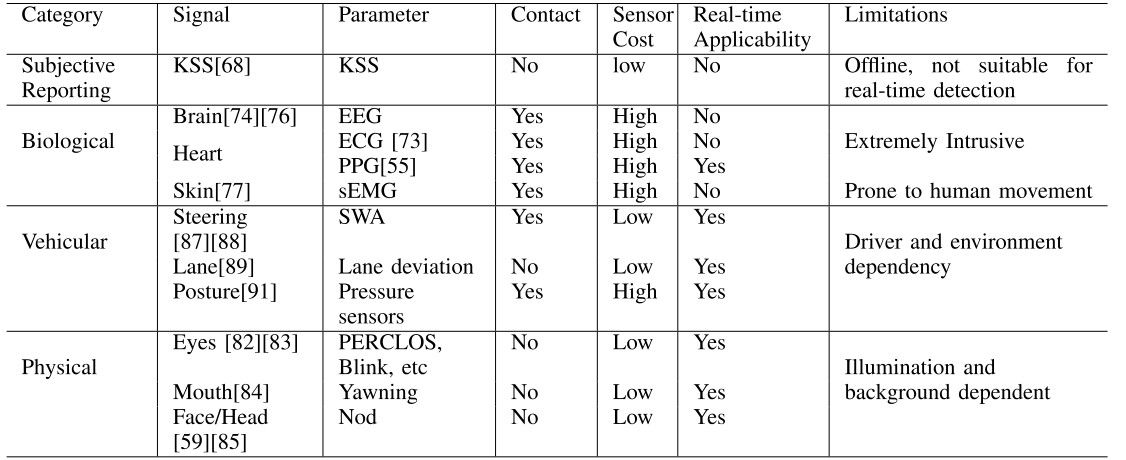
\includegraphics[width=6in]{example/comparison.jpg}
\label{table:1-4}
%\end{minipage}

\end{table}

\section{疲劳分析方法和检测指标}

前面介绍了多种疲劳检测的特征,主要分成3类:生物电信号特征,行为特征,车辆特征。其中生物电信号特征主要通过心电信号,脑电信号,肌电信号,眼电信号来提取;行为特征包括眼睛,嘴巴,脸部和头部;而车辆特征主要包括方向盘转角,车道偏离和驾驶员姿势变化。本小节我将大致介绍一下基于上述这些特征的分析方法。而在第二章我会具体介绍分析方法中涉及到的算法和模型。

\subsection{基于行为特征和车辆特征的分析方法}

将行为特征与车辆特征相结合进行疲劳检测,可以大大提高疲劳检测的准确性。Cheng等人在2012年《\href{https://xueshu.baidu.com/usercenter/paper/show?paperid=40e6cefe0fa8b0e382379eef9d105952&site=xueshu_se}{Driver
drowsiness detection based on multisource information}》 一文中,选择了8 个特征来进行疲劳检测,包括PERCLOS、眨眼率、最大闭眼时间、非转向百分比、on-centre 行车百分比(LCP 吗?)、方向盘转角标准差、车道位置标准差,其中二十名参与者参加了这个实验。此外,还开发了一个多源数据融合模型,融合来自司机和车辆的信息。对于疲劳估计,单使用车辆特征,检测精度为81.9$\%$;单使用驾驶员行为特征,检测精度为86.9$\%$,而融合了行为特征与车辆特征,检测精度为90.7$\%$。 疲劳是根据方差分析(ANOVA)和约翰斯嗜睡量表(JDS) 作为真实标签来确定的。

在2015年《\href{https://xueshu.baidu.com/usercenter/paper/show?paperid=50ad15f8eb9411555a57acd85d167dff&site=xueshu_se&hitarticle=1}{A Self-Adaptive Dynamic Recognition Model for Fatigue Driving Based on Multi-Source Information and Two Levels of Fusion}》一文中,作者提出了一种自适应的动态识别模型,利用最有效的特征进行特征融合来检测疲劳。该模型使用的行为特征包括眨眼频率(BF)、闭眼时长(ECD)、睁眼平均水平(MEOL)和打哈欠频率(YF)。车辆特征包括非转向率(PNS)、 转向角度标准偏差(SDSA)、异常车道偏离频率(FALD)和车速标准差(sdv)。基于Takagi-Sugeno模糊神经网络(T-SFNN) 进行特征融合。仅使用车辆特征,系统的准确率为90.8 $\%$,而仅使用面部特征,疲劳检测准确率为91.6$\%$。如果融合了所有的行为特征和车辆特征,疲劳检测精度达到92.1$\%$,但如果融合最有效的特征,疲劳检测精度可以达到93.8$\%$ 。这表明,只融合有效的特征而非融合所有可能的特征显得更为重要。

\subsection{基于行为特征和生物电信号的分析方法}

直接从驾驶员中提取特征有可能得到精度高的预测结果,在2015 年《\href{https://xueshu.baidu.com/usercenter/paper/show?paperid=18ca7cad0c2f50c8fd84edb4cf68228e&site=xueshu_se&hitarticle=1}{Driver Alertness Monitoring Using Fusion of Facial Features and Bio-Signals}》一文中,作者提出了基于Eye和PPG特征的DBN 模型。作者从驾驶员上提取眼部特征和PPG信号,并通过无线方式发送到基于android系统的智能手机上,这两类特征输入到深度置信网络(DBN), DBN最终会输出一个概率值,代表司机的疲劳水平。在真实驾驶实验中,10名参与者接受了测试,实验分析表明:与单纯使用生理或生物电特征相比,生理和生物电特征融合的疲劳检测效果更好。

\subsection{基于生物电信号和车辆特征的分析方法}

生物电信号和车辆特征的融合吸引了研究人员对驾驶员疲劳检测的研究。Lee等人在2015 《\href{https://xueshu.baidu.com/usercenter/paper/show?paperid=7515e7f9ea210a19031c7d2779900c36&site=xueshu_se}{Smartwatch-based driver alertness monitoring with wearable motion and physiological sensor}》一文中提出了一种融合PPG和方向盘转角的疲劳检测方法,该方法根据智能手表内置的陀螺仪估计方向盘转向运动,通过蓝牙将PPG 传感器数据传输到智能手表。在模拟实验中,采用视觉线索和KSS作为ground truth,采用基于移动的支持向量机(M-SVM) 对驾驶员状态进行分类,最终预测准确度可达到95.8$\%$ 。该实验在模拟环境下准确度很高,但该方法没有在真实道路环境上接受测试。

\subsection{基于生物电、行为和车辆特征的分析方法}

考虑到上面三种模型的预测效果,我们可以感受到,通过生理、车辆和生物电信号的融合来检测驾驶员疲劳会是一种自然的研究思路。在2014年《\href{https://xueshu.baidu.com/usercenter/paper/show?paperid=8b16b46bd02a42af28065c279838ef5b&site=xueshu_se&hitarticle=1}{Data
fusion to develop a driver drowsiness detection system with robustness to signal loss}》一文中,作者使用决策模块,对三个神经网络的决策进行融合,而每个神经网络使用不同的特征来检测疲劳。作者利用眼睛状态、方向盘转角(SWA)、心电信号、脑电信号、表面肌电信号进行疲劳检测,其中12 个人参与了模拟实验,实验得出该系统最终预测准确率为94.63$\%$。

表\href{table:1-5}{1-5}对以上分析方法进行了总结

\begin{table}[!htp]

\centering
%\begin{minipage}[t]{5in}
\caption{分析方法汇总}
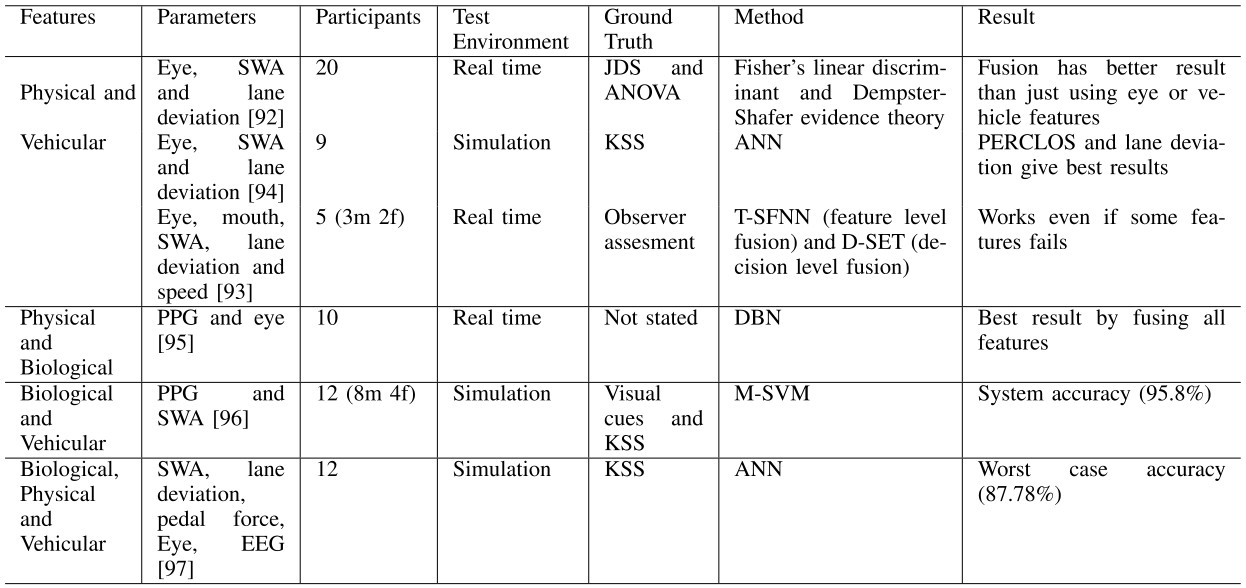
\includegraphics[width=6in]{example/method.jpg}
\label{table:1-5}
%\end{minipage}

\end{table}

\subsection{疲劳检测的客观指标}

前面我们介绍了疲劳检测相关数据及对应的特征,介绍了疲劳检测的分析方法,但在此之前,我还是有必要介绍一下疲劳检测的客观指标。假设我们现在可以利用某种传统方法,或者利用卷积神经网络对某类带标签的数据集进行特征抽取(标签可以通过KSS,或PERCLOS等视觉特征进行标注),接着使用某个模型对特征进行预测分析,最终我们会得到一系列的疲劳预测结果。一般我们会使用准确度(Accuracy),精度(Precision),召回率(recall) 等作为分类指标,但是个人觉得这些指标在有标签分类上效果好,但对于无标签分类上应用比较有限,主要原因是对于心率变异性(HRV)和不同频率的脑电波($\alpha$ 波、$\beta$ 波、$\theta$ 波、$\delta$ 波),它们在医学方面的研究已经日渐成熟,可以通过该特征具有的特性直接预测疲劳程度,所以接下来要介绍的客观指标主要和某些特征有关。在研究中,我们可以利用这些指标作为某些特征的判断基准,辅助监督学习模型进行疲劳估计,进而提高检测精度。

\subsubsection{生物电信号指标}

1、HRV

心率变异性(Heart Rate Variability, HRV)用于描述自主神经系统交感神经与副交感神经分支的传出活动引起的心率搏动变化,直观表现为连续心跳之间的时间间隔,通常可以通过计算BVP信号连续峰值之间的差值得到。HRV是测量应激水平的指标,应激和疲劳虽然不等同但是相互关联,在实验条件的严格控制下,HRV 可以用于评价脑力疲劳状态(参考《\href{https://xueshu.baidu.com/usercenter/paper/show?paperid=022a05752137ea8cb415ac94f27421d0&site=xueshu_se&hitarticle=1}{基于心率变异性的精神疲劳的研究}》) 。诱发脑力疲劳的方式主要有连续长时间的认知任务操作和睡眠剥夺(参考《\href{https://xueshu.baidu.com/usercenter/paper/show?paperid=8288f753c5b84d6728391325a90bb7ba&site=xueshu_se&hitarticle=1}{脑力疲劳的实验室诱发模型和评价手段研究进展}》) 。

诱发脑力疲劳的方式主要有连续长时间的认知任务操作和睡眠剥夺。国内外已有不少学者对采用HRV评价不同方式诱导的脑力疲劳状态作了研究。李延军等通过设计读书和笔算两种脑力疲劳实验发现随着读书或笔算过程中疲劳程度的增加,心率下降而HRV 上升,并且认为以工作绩效检测脑力疲劳具有局限性。通过睡眠剥夺的方式诱发脑力疲劳实施性高且效果显著。Chua等研究了受试者在40 h的睡眠剥夺过程中每隔两小时采集到的ECG 信号的HRV指标和精神运动警觉性任务,结果发现HRV指标可用于监测疲劳,并可作为预测人体困倦的指标。

HRV具有昼夜节律性,白天时交感神经活性较强,夜晚时副交感神经活性较强。HRV功率谱的低频功率(Low Frequency Power, LF)反映交感神经活性,高频功率(High Frequency Power, HF)反映副交感神经活性,LF/HF反映交感神经和副交感神经的均衡性(参考《\href{https://kns.cnki.net/kcms/detail/detail.aspx?dbcode=CJFD&dbname=CJFD2000&filename=ZJCY200002034&v=6qyW5%25mmd2Fqipk1z5EsYGOVGp3krgokDUYjpqpntc63glD9%25mmd2BqO5mYMAsQkXAR8sIv6tB}{健康人心率变异的昼夜节律分析}》) 。虽然国内外不少学者对由睡眠剥夺诱导的脑力疲劳状态的HRV进行了研究分析,但考虑HRV 昼夜节律性的研究较少。Quintana 等认为24 h 的实验室睡眠剥夺不会改变健康年轻男性仰卧位的高频HRV。

取自\href{https://xueshu.baidu.com/usercenter/paper/show?paperid=b0ea6808d2959e6a495e1ca285ed72d5&site=xueshu_se&hitarticle=1}{基于心率变异性的脑力疲劳检测}


2、HR

许多研究人员认为,心率(HR)对于不同任务具有敏感性,并且对心率的分析较为简单而又直接
\footnote{1984 - Inflight evaluation of four measures of pilot workload. Human Fact. Ergonom \quad \url{https://xueshu.baidu.com/usercenter/paper/show?paperid=4a505cb57cd0f12373f3827ec2a1eea7&site=xueshu_se}}。
Wilson 和O'Donnell
\footnote{1988 - Measurement of operator workload with the neuropsychological workload test battery \quad \url{https://xueshu.baidu.com/usercenter/paper/show?paperid=b1ba49e4b3c1c2e6072df39296608219&site=xueshu_se&hitarticle=1}} 结合其他研究者的研究成果,认为HR信号是反映不同任务下心理和生理负荷水平的整体指标;
Hart
\footnote{1990 - Workload Assessment and Prediction \quad \url{https://xueshu.baidu.com/usercenter/paper/show?paperid=49d5f6b46766233faaafe9308a8fd685&site=xueshu_se&hitarticle=1}} 等也认为,HR信号反映了各种因素对操作员的综合影响,比如任务和情绪等; Riemersma et al.
\footnote{1976 - Performance Decrement During Prolonged Night Driving \quad \url{https://xueshu.baidu.com/usercenter/paper/show?paperid=eabda605ad0ca65dcb1814bac6f04b75&site=xueshu_se}} 发现驾驶员长时间驾驶后HR会降低;
Hartley et al.
\footnote{1994 - Indicators of fatigue in truck drivers \quad \url{https://xueshu.baidu.com/usercenter/paper/show?paperid=2fb37c1ac987ae750c94d33ad3dd7d0b&site=xueshu_se&hitarticle=1}} 认为HR变化有助于驾驶疲劳检测。

HR信号是随机信号。因此,为了真实反映HR的变化,需要对原始HR数据进行一定的过滤处理。即使在相同情况下,由于个体差异,司机的HR基准也存在差异。为了更好地反映HR的变化,有学者
\footnote{2020 - Fatigue driving detection method for low-voltage and hypoxia 4 plateau area: A physiological characteristic analysis approach \quad \url{https://xueshu.baidu.com/usercenter/paper/show?paperid=19750260gk3u0270qe7g0gk0hj383393&site=xueshu_se&hitarticle=1}} 提出用HR速率(A)来描述驾驶员的心理生理变化。其中A是某一时刻的HR值$H(T_N)$减去前一分钟的HR值$H(t_{n-1})$与前一分钟的HR值$H(t_{n-1})$ 的比值。

\begin{equation}
A = \frac{{H(t_n)} - H{(t_{n-1})}}{H{(t_{ncot -1})}} * 100 \%
\end{equation}

3、SpO2

氧气是维持人类生命最重要的物质之一,有研究发现,血液中的氧含量会随着疲劳而降低。因此,对于疲劳驾驶,实时评估人体组织在疲劳状态下的血氧饱和度(SpO2)具有重要的指导意义。有很多研究表明,驾驶员体内的SpO2会随着驾驶时间和疲劳程度的增加而降低(\footnote{2002 - Blood pressure and heart rate variability in taxi drivers on long duty schedules\url{https://xueshu.baidu.com/usercenter/paper/show?paperid=dffd6debc53746876da216842a6305c4&site=xueshu_se&hitarticle=1}})。 在低压低氧高原环境下,由于地形的特殊性,驾驶员疲劳驾驶的风险高于平原地区,相应的后果也会更严重,因此值得更多关注。

有学者\footnote{2020 - Fatigue driving detection method for low-voltage and hypoxia
4 plateau area: A physiological characteristic analysis approach \quad \url{https://xueshu.baidu.com/usercenter/paper/show?paperid=19750260gk3u0270qe7g0gk0hj383393&site=xueshu_se&hitarticle=1}} 通过计算SpO2和疲劳程度KSS的皮尔逊相关系数,发现仅通过SpO2 并不能准确预测疲劳,主要原因是个体差异性,即使在相同的情况下,驾驶员的SpO2基准也存在差异。为了更好地反映SpO2的变化,作者提出用SpO2 速率(B) 来描述驾驶员的心理生理变化。B 是某一时刻的SpO2值$O(t_n)$减去前一分钟的SpO2值$O(t_(n-1))$与前一分钟的SpO2 值$O(t_(n-1))$的比值。

\begin{equation}
A = \frac{{O(t_n)} - O{(t_{n-1})}}{O{(t_{n -1})}} * 100 \%
\end{equation}


\subsubsection{面部行为指标}

面部行为指标主要包括:BF, YF, ABT和PERCLOS,这些指标可以通过多种方式计算得到。

1、EAR

眼睛的纵横比(Eye Aspect Ratio, EAR)数值等于眼睛纵向界标与横向界标之间的欧氏距离比值,以左眼为例,其计算如式\href{2.1}{2.1}所示,其中P代表人眼特征点,其下标表示图\href{2-4}{2-4}中的特征点编号。右眼的 EAR值计算同理。

\begin{figure}[!htp]

\centering
%\begin{minipage}[t]{5in}
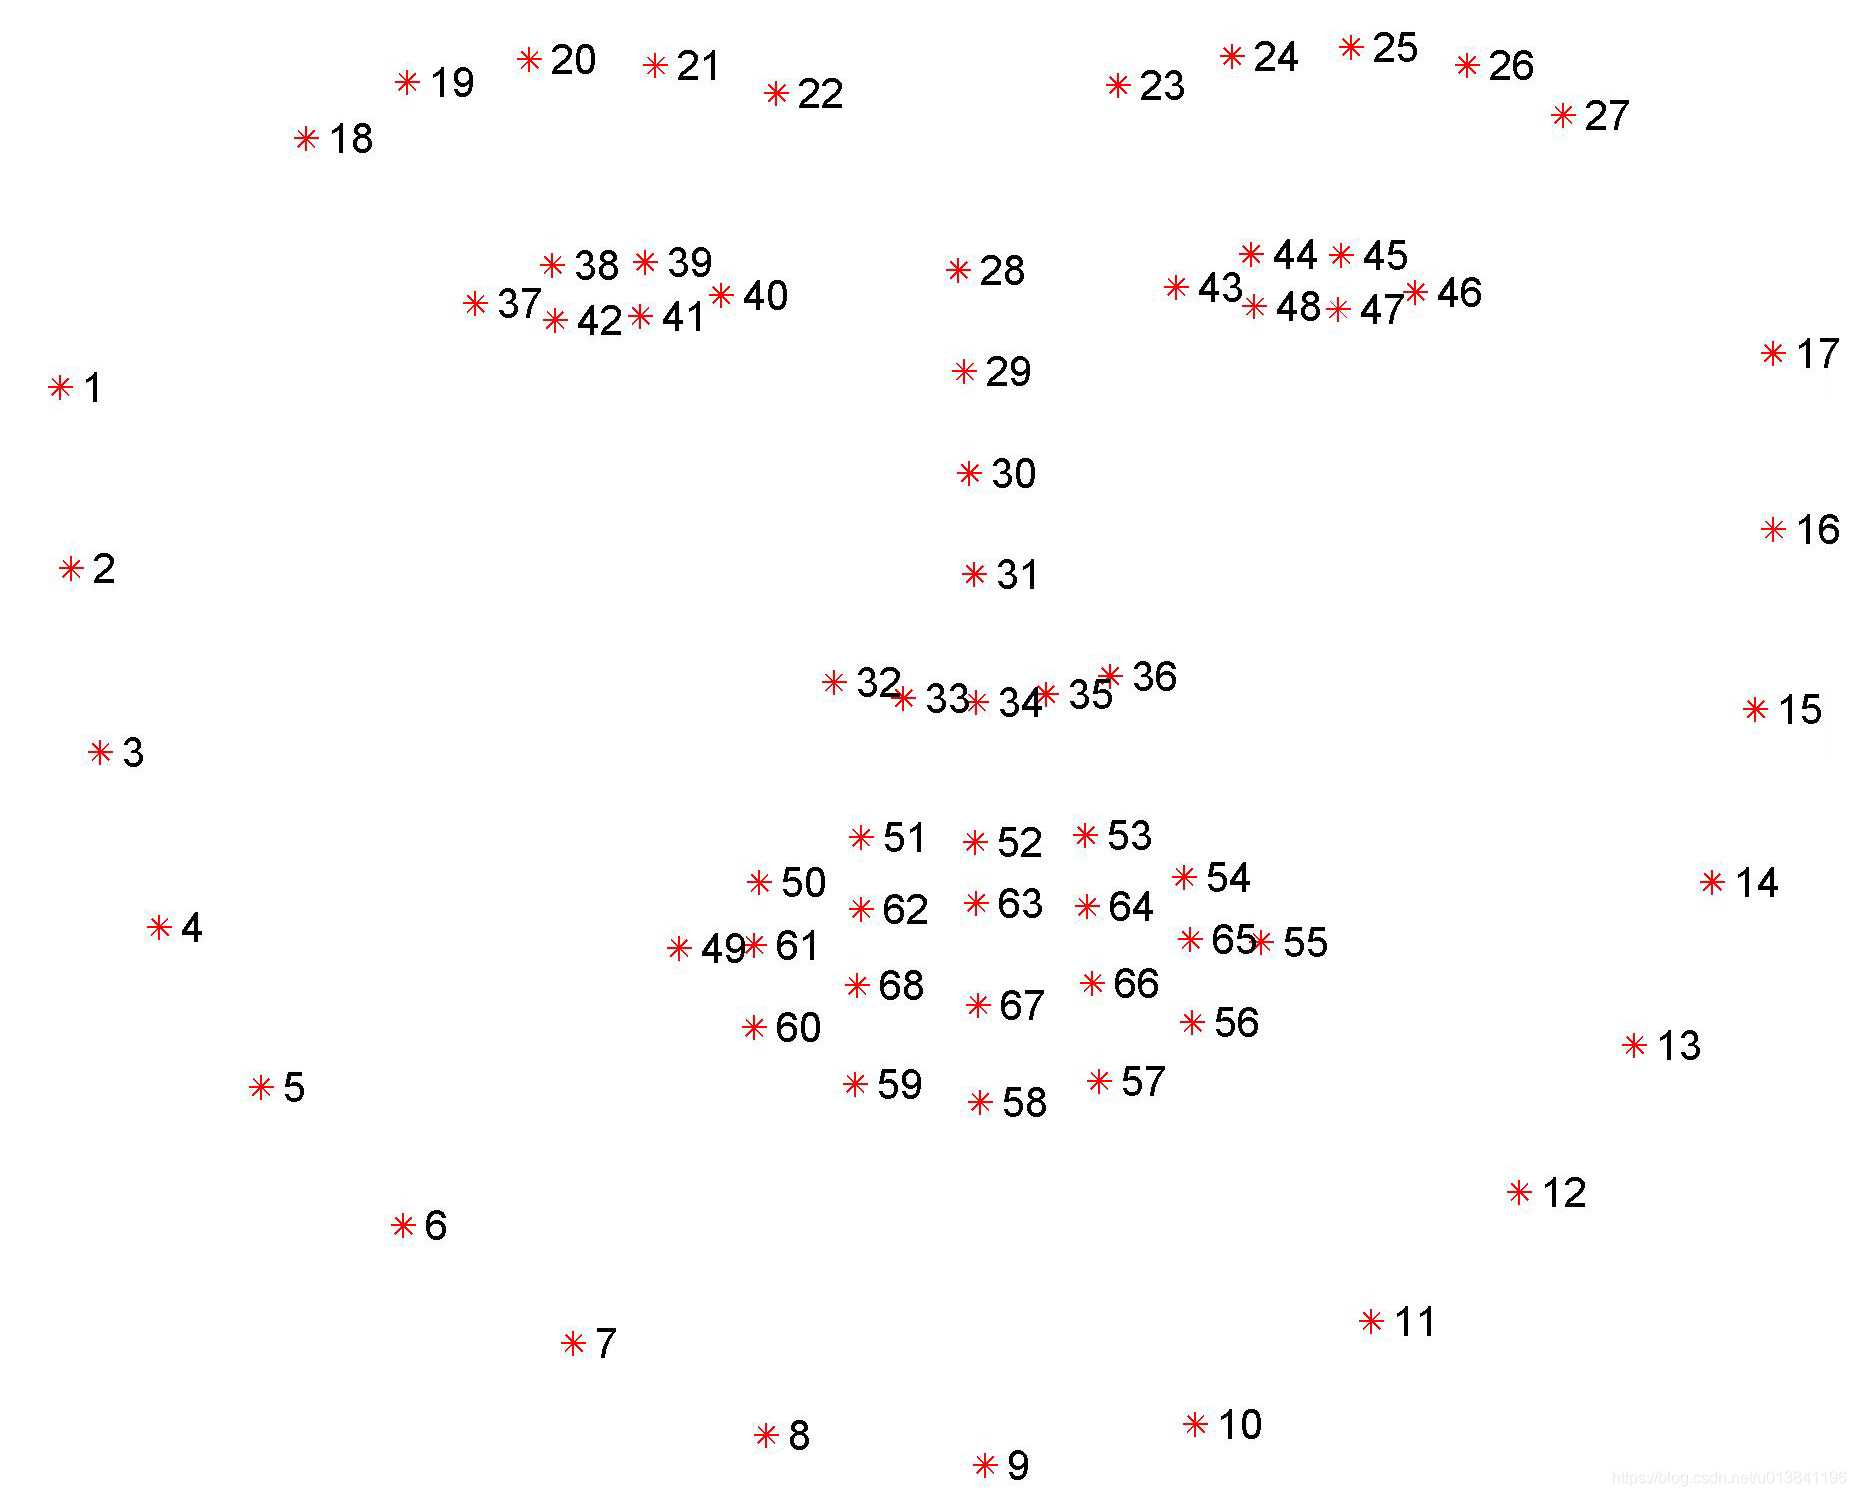
\includegraphics[width=4in]{example/landmark.jpg}
\caption{dlib 68个关键点}
\label{table:2-4}
%\end{minipage}

\end{figure}

图\href{2-5}{2-5}记录了两次眨眼过程的 EAR 值的变化。当人眼睁开时,EAR 值基本保持稳定;当人眼闭合时,EAR 迅速下降,理论上会接近于零;当人眼再次睁开时,EAR 值恢复到稳定的状态。EAR 值的"稳定—突然下降—恢复"稳定的过程反映了人的一次眨眼全过程。因此,一个复杂图像处理问题被转化成了眼睛特征点之间距离的比例关系。

受限于算法标定的准确度,即使在没有眨眼的情况下,EAR 数值仍然会发生明显的波动,如图 4 中的睁眼阶段。为了避免 EAR 数值波动引起的眨眼误判,当捕捉到连续 2 $\sim$ 6 帧的 EAR 值低于某个 EAR 阈值时,才认为被测对象进入了眨眼状态,记录为一次眨眼。连续帧数和阈值都需要根据摄像设备进行确定。连续帧数取决于摄像机的帧率。帧率越高的摄像机在一次眨眼过程中能捕捉到的低于阈值的帧数就越多,对检测对象是否眨眼的判定也就越准确;而相反,如果对低帧率的摄像机选用较多的连续帧数判定,则会导致眨眼次数的漏报,影响检测精度。

考虑到每个人 EAR 阈值存在个体差异,本研究中以检测对象前 $30$s 的视频作为样本,计算其中每一帧的 EAR 值,统计得出 EAR 中位数。因为一个人眨眼的帧数一般不会超过总帧数的 15$\%$,中值一定反映的是睁眼状态下的 EAR。考虑到睁眼状态下 EAR 的数值波动,本研究取 $0.8$ 倍的 EAR 中值作为 EAR 阈值。

\begin{figure}[!htp]

\centering
%\begin{minipage}[t]{5in}
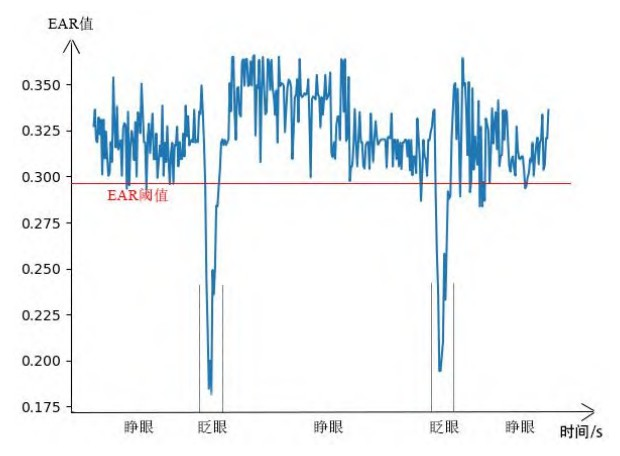
\includegraphics[width=4in]{example/EAR.JPG}
\caption{睁眼与眨眼过程中的EAR值曲线}
\label{table:2-6}
%\end{minipage}

\end{figure}

\begin{equation}
EAR = \frac{\vert P_{38} - P_{42} \vert + \vert P_{39} - P_{41} \vert}{2 \vert P_{40} - P_{37}\vert}
\end{equation}

2、MAR

嘴巴纵横比(Mouth Aspect Ratio, MAR)的定义与 EAR 相似,其计算如式\href{2.2}{2.2}所示,其中 m 代表人嘴特征点,其下标表示图\href{2-4}{2-4}中的特征点编号。和 EAR 指标相似,判断是否打哈欠的依据也是连续 10 $\sim$ 60 帧的 MAR 值大于某个阈值。连续帧数的取值同样依据视频的帧率确定;阈值的选取考虑个体差异,取为前 30s 的视频的 MAR 值中位数的 1.5 倍。

\begin{equation}
MAR = \frac{|m_{51} - m_{59}| + |m_{53} - m_{57}|}{2|m_{55} - m_{49}|}
\end{equation}

3、BF,YF

眨眼频率(Blink Frequency, BF)和哈欠频率(Yawn Frequency, YF)是疲劳估计的重要指标。
在《\href{https://kns.cnki.net/kcms/detail/11.5823.tu.20210201.1703.039.html}{基于计算机视觉技术的施工机械操作员疲劳作业检测方法}》一文中,作者通过设置EAR阈值,计算BF和YF。

\begin{figure}[!htp]

\centering
%\begin{minipage}[t]{5in}
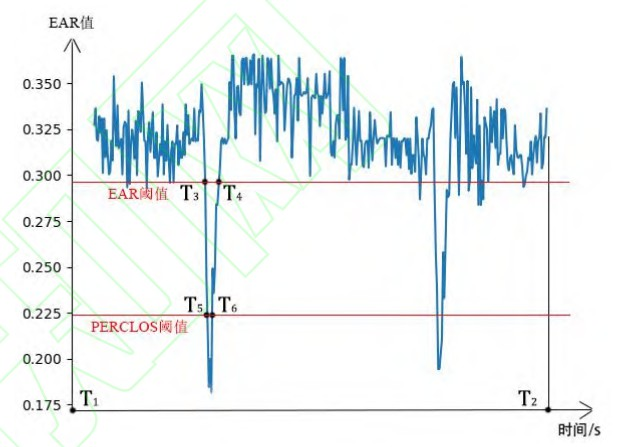
\includegraphics[width=4in]{example/indicator.JPG}
\caption{疲劳指标计算原理}
\label{table:2-6}
%\end{minipage}

\end{figure}

BF计算如式\href{2.3}{2.3},其中,n 为累计眨眼次数。同理可得YF,其中各参数的含义如图\href{2-6}{2-6}所示。
\begin{center}
\begin{equation}
BF = \frac{n}{T_{2} - T_{1}}
\end{equation}
\end{center}

4、ABT

平均眨眼时长(Average Blink Time, ABT)是疲劳估计的重要指标。
在《\href{https://kns.cnki.net/kcms/detail/11.5823.tu.20210201.1703.039.html}{基于计算机视觉技术的施工机械操作员疲劳作业检测方法}》一文中,作者通过设置EAR阈值,计算ABT。ABT计算如式\href{2.4}{2.4},其中各参数的含义如图\href{2-6}{2-6}所示。
\begin{center}
\begin{equation}
ABT = \frac{\sum(T_4 - T_3) }{n}
\end{equation}
\end{center}

5、PERCLOS

眼睑闭合时间百分比(Percentage of Eyelid Closure time,PERCLOS)是疲劳估计的重要指标。
在《\href{https://kns.cnki.net/kcms/detail/11.5823.tu.20210201.1703.039.html}{基于计算机视觉技术的施工机械操作员疲劳作业检测方法}》一文中,作者通过设置EAR阈值,计算PERCLOS(如式\href{2.5}{2.5})。图\href{2-6}{2-6}中的 EAR 阈值取前 30 秒视频中 EAR 中值的 0.8 倍;PERCLOS 阈值计算如式\href{2.6}{2.6}。其中 p 为 PERCLOS 阈值,e 为 30 秒后的前三次眨眼过程中 EAR 最小值的平均数,m 为第 0 秒至 30秒后的第三次眨眼结束,这段时间内的 EAR 中值。
\begin{center}
\begin{eqnarray}
PERCLOS = \frac{\sum(T_6 - T_5) }{T_2 - T_1} \\
p = e + 0.2 * (m - e)
\end{eqnarray}
\end{center}

在PERCLOS计算中,闭眼时间的计算较为关键,有些研究者通过EAR计算闭眼时间,有些学者则是通过检测瞳孔的大小判断是否闭眼,进而计算闭眼时间。
在
《\href{https://www.baidu.com/link?url=rLtX9O68zFaOoixH2L36t_Tukm6iwagyZgLiTajxaa9ZjZRDzOhUYp5VlGUJxjfwj5ZdsT4xsrv8GXa2g_oe-fmSsP0BWbzEkzLkdlDj6cN-ddXWcugdKsn8POeyqXpQPKGtqu5FfYIJ-DqI1rg7cF9WRFj9gW-A6kpojIQOJ6dZ_68pC_R8cVd5bY1jW0LA&wd=&eqid=8bac1342000bb654000000056040c52e}{Fatigue detection based on multi-feature fusion of fatigue behavior}》一文中,作者将疲劳划分为3类:正常疲劳,一级疲劳,二级疲劳,并且使用PERCLOS(通过瞳孔纵轴长度判断眼睛状态),嘴巴张合程度(通过嘴巴张开面积进行计算)和点头频率(通过脸部位置判断头部运动状态)作为疲劳检测的指标,疲劳判断准则如表\href{table:2-6}{2-6} 所示。
PERCLOS计算规则如下:假设检测时间$I > 3s$,计算得到的闭眼时间为T,因此闭眼时间百分比$f = \frac{T}{I} \cdot 100\% $

\begin{table}[!htp]

\centering
%\begin{minipage}[t]{5in}
\caption{分析方法汇总}
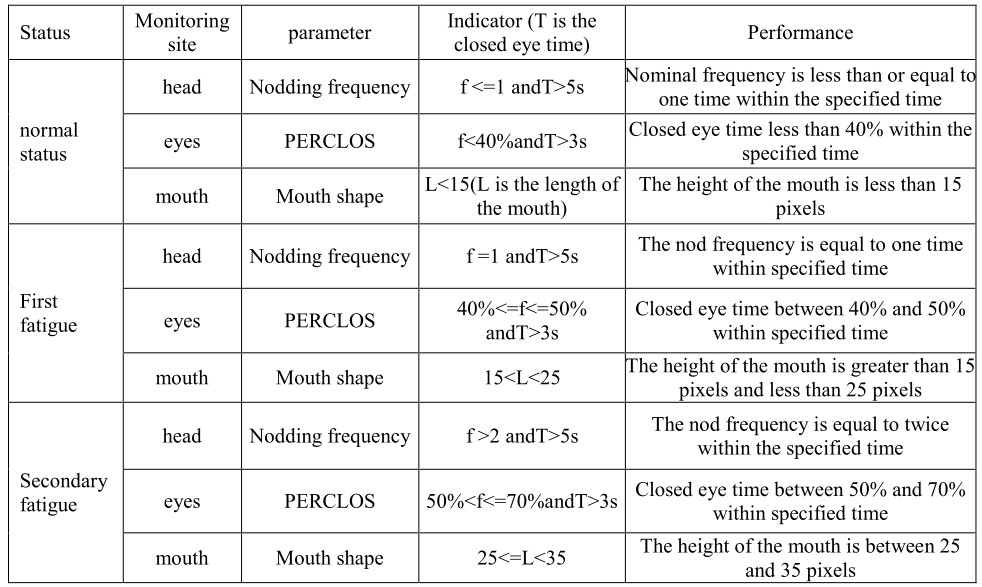
\includegraphics[width=6in]{example/fatigueLevel.JPG}
\label{table:2-6}
%\end{minipage}

\end{table}

\subsubsection{车辆指标}

\subsection{谈谈我的理解}

在我们生活的世界,到处都存在特征,对于不同物种,它们观察到的特征是不一样的,这主要和生物构造有关,比如变色龙看到的东西和我们看到的东西是不一样的。即使是相同物种,它们观察的特征也有所区别,以人为例,对于同一幅画,不同个体有各自的主观理解,这主要和我们之前所习得的特征在大脑中构建的网络结构有关。

1、特征是什么?

在我看来,特征可以分为主观特征和客观特征。

主观特征是人类通过直接或间接经验从客观事物上学习到的特征,这些特征是人类认识客观世界,构建自己知识体系,并用自己知识体系解释客观现象的关键性输入。但主观特征不足之处在于,这些特征可能会由于自身认知存在的偏见导致特征在进一步提取过程中不是那么客观,这时就需要通过例证或实践来验证自己归纳的特征的客观性。

而客观特征可以理解成事物的客观属性、而多种客观特征的组合构成了事物的本质属性,它有微观和宏观的区别。它可以是人类不断抽象化自己主观特征的智慧结晶,也可以是计算机深度学习过程的产物。这些客观特征,一方面它是对某个客观事物的反映。假设我们已知这些信息:四条腿行走,脑重和体重比为0.66$\%$,那么至少我们可以推断出它不是人,因为正常人不四条腿走路,婴儿的脑重和体重比约为11.71$\%$。 另一方面,特征也可以反映客观事物的行为,如果把手看做是人的一个特征的话,那么他大概率可以握拳。

下面这段话作者从语言特征和文化特征的关联性出发,解释东西方语言或文化的本质特征\footnote{英汉对比研究 \quad \url{https://book.douban.com/subject/5297697/}}。

\begin{example}
\\
在寻找语言特征或文化特征时,个性与共性、部分现象与普遍现象的界定有个量化和定性的问题。如果大量的调查研究证明,某种语言现象或文化现象拥有绝大多数的例证,这些例证又足以证明在该语言中或该文化中的本质特征,并经得起例外的反证,这就可以确定其为特征或特点,否则就难以定论。语言与文化所表现的现象十分复杂,涉及的知识非常广泛,研究其特征及相互关联时应作具体、动态、多角度的分析,并用大量可靠的例证加以论证,不能轻易一概而论,不能为了得出某种预想的结论而采取“一刀切”的态度、忽视可能还有反面的例证。
\\
\end{example}


2、对于特征的分析方法有哪些?

在我看来,特征可以用来定性分析,也可以用来定量分析。对于定性和定量,网上有直观的解释
\footnote{\url{https://wenku.baidu.com/view/d66ae51dc5da50e2524d7f45.html}}:
定性是指用文字语言描述,定量是指用数学语言描述。定性分析与定量分析应该是统一的,相互补充的,定性分析是定量分析的基本前提,没有定性的定量是一种盲目的、毫无价值的定量,定量分析使之定性更加科学、准确,它可以促使定性分析得出广泛而深入的结论。

在人为决策过程中,我们可以通过一系列特征组合,凭直觉和经验,判断是猫还是人,这就是定性分析。我们还可以依据数据统计量(样本中心距,样本均值等)作为特征建立数学模型,并用数学模型计算出分析对象的各项指标及其数值关系,进行定量分析。

3、定量分析由哪几部分构成?

定量分析 = 具有统计特性数据 + 数学模型 + 指标。

1) 统计特性

统计特性又称统计特征,统计特征有数量特征和属性特征之分,其中数量特征又有计量特征和计数特征之分。数量特征可以直接用数值来表示,例如,元件的大小尺寸、小麦的株高等均是计量特征;而夏季暴雨的次数、一平方米布料上疵点的个数是计数特征;属性特征不能直接用数值来表示,如产品是否为合格品、每个人的性别等,特征就是要考察的指标。

数据分布特征可以从集中趋势、离中趋势及分布形态三个方面进行描述 \footnote{\url{https://blog.csdn.net/qq_36330643/article/details/77197235}}。

\begin{enumerate}[label=\circled{\arabic*}]
    \item 平均指标是在反映总体的一般水平或分布的集中趋势的指标。测定集中趋势的平均指标有两类:位置平均数和数值平均数。位置平均数是根据变量值位置来确定的代表值,常用的有:众数、中位数。数值平均数就是均值,它是对总体中的所有数据计算的平均值,用以反映所有数据的一般水平,常用的有算术平均数、调和平均数、几何平均数和幂平均数。
    \item 变异指标是用来刻画总体分布的变异状况或离散程度的指标。测定离中趋势的指标有极差、平均差、四分位差、方差和标准差、以及离散系数等。标准差是方差的平方根,即总体中各变量值与算术平均数的离差平方的算术平方根。离散系数是根据各离散程度指标与其相应的算术平均数的比值。
    \item 矩、偏度和峰度是反映总体分布形态的指标。矩是用来反映数据分布的形态特征,也称为动差。偏度反映指数据分布不对称的方向和程度。峰度反映是指数据分布图形的尖峭程度或峰凸程度。
\end{enumerate}

比较重要的几个关键数据:
\begin{enumerate}[label=\circled{\arabic*}]
    \item 均值。
    \item 加权算数均值。
    \item 截断均值。
    \item 中位数。
    \item 数据倾斜,均值大于中位数,正倾斜;均值小于中位数,负倾斜。
    \item 中列数。
    \item 百分位数,中位数是第50个百分位数,第一个四分位数Q1是第25个百分位数,第三个四分位数Q3是第75 个百分位数。
    \item 中间四分位数极差IQR = Q3-Q1。
    \item 众数。
\end{enumerate}

数据散布程度度量:
\begin{enumerate}[label=\circled{\arabic*}]
    \item 极差,最大值和最小值之间的差异。
    \item 绝对平均偏差,AAD(absolute average deviation)
    \item 中位数绝对偏差  MAD(median absolute deviation)
    \item 四分位数极差   IQR(interquartiles range)
\end{enumerate}

2) 数学模型

谈到模型,这里我们给出模型的通用性解释:模型是对现实的抽象,它允许我们剥离细节,并从特定的角度来观察实体或概念。数学模型则是用数学语言描述的一类模型,小到一个数学公式、神经网络中一个卷积模板,大到整个神经网络,都可以看做是一个模型,不同模型有不同的特征分析方法,在机器学习中,模型可以看做是数据 + 算法\footnote{\url{https://zhuanlan.zhihu.com/p/162086776}}。 根据模型的功能,还可以将模型分成生成模型和判别模型\footnote{\url{https://www.zhihu.com/question/20446337/answer/165277084}}。 生成模型是对联合概率分布建模,判别模型是对边缘概率分布建模。常见的判别模型有:线性回归模型、支持向量机SVM、逻辑斯蒂回归模型、决策树等;常见的生成模型有朴素贝叶斯模型、隐马尔可夫模型HMM、 混合高斯模型等。

3) 指标

对于定量分析,如果没个准确的判断标准是不行的,量的大小无法得到确定。指标的通用性解释是指在预期中打算达到的指数、规格、标准,在实际的统计工作和统计理论研究中,往往直接将说明总体数量特征的概念称为指标。而我理解的指标是指在一定取值范围内有意义的数量特征或数量特征的集合,是反映数量特征和实体属性,或和实体间关系的标准。比如PERCLOS,HR指标可以反映人的疲劳程度,某地区平均从业人数可以反映该地区的繁荣水平。指标可通过直接计算得到(比如网站平均访问量,注册用户数,准确率,精确率等),也可间接计算得到(PERCLOS,EFF影响因子等综合指标)。\\

4、神经网络和定量分析

现在我们可以分析一下,神经网络是不是属于定量分析的范畴。虽然神经网络是一个数学模型,但它所习得的特征不是通过统计得到的,因此在量上就无法确定。没有了"量",指标就无从下手,也就没有了"定"的概念,因此神经网络不属于定量分析的范畴。在我看来,神经网络就像人的大脑一样,对于事物的理解处于定性分析的层面,它通过单一的特征(单一尺度特征图)或者一系列的特征组合(不同尺度特征图的融合),凭直觉和经验(梯度下降等优化算法),判断是猫还是人。

但是对于神经网络模型的评估就属于定量分析的范畴了。以二分类问题为例,通过对分类正确的样本进行统计,可以得到各项指标:准确率,精确率,召回率等。通过这些指标,我们可以绘制ROC 曲线,计算AUC面积,进而实现对神经网络模型的评估\footnote{\url{https://www.jianshu.com/p/1afbda3a04ab}}。

\section{疲劳检测开源数据集}

\subsection{Nthu-DDD数据集}

\href{http://cv.cs.nthu.edu.tw/php/callforpaper/datasets/DDD/}{Nthu-DDD 下载地址}

\href{https://xueshu.baidu.com/usercenter/paper/show?paperid=785509793c585892cce84b2507683812&site=xueshu_se}{Nthu-DDD 论文地址:Driver Drowsiness Detection via a Hierarchical Temporal Deep Belief Network}

Nthu-DDD是新竹大学计算机视觉实验室收集的驾驶员嗜睡视频数据集,整个数据集(包括训练、评估、测试数据集)包含36名不同种族,戴眼镜(太阳镜)和不戴眼镜(太阳镜)的参与者,在白天和夜间的光照条件下,在各种模拟驾驶场景下,包含正常驾驶、打哈欠、慢眨眼、打瞌睡、突然大笑等。参与者坐在椅子上玩模拟方向盘和踏板,进行普通的驾驶游戏;同时,他们会在实验者的指导下做出一系列不同的面部表情。整个数据集的总时长约为9个半小时。

训练数据集包含5种不同场景(裸脸、戴眼镜、夜间裸脸、戴夜视镜、戴太阳镜)共18个参与者。对于每个参与者,需要记录他/她打哈欠,点头和慢眨眼等动作序列,每个记录大约长达1 分钟。其中有两个最重要的场景(嗜睡场景和非嗜睡场景)对应的动作序列,即嗜睡相关动作组合(打哈欠、点头、眨眼速度慢)和非嗜睡相关动作组合(说话、大笑、看两边),每个记录大约长达1.5分钟。评估和测试数据集包含90个驾驶视频(来自其他18个参与者),在不同的场景下记录参与者困倦和非困倦状态。相同场景下的不同动作如图\href{figure:2-8}{2-8} 所示,不同场景下的相同动作如图\href{figure:2-9}{2-9}所示。该数据集主要研究在不同场景下不同动作组合所反映的嗜睡程度。

\begin{figure}[!htp]

\centering
%\begin{minipage}[t]{5in}
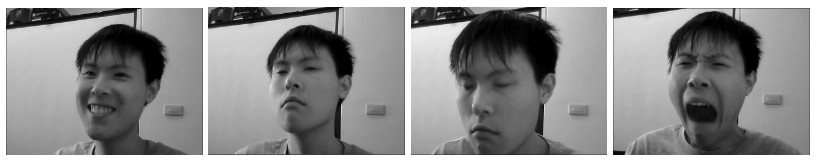
\includegraphics[width=5in]{example/NTHU1.jpg}
\caption{相同场景下的不同动作}
\label{figure:1-7}
%\end{minipage}

\end{figure}

\begin{figure}[!htp]

\centering
%\begin{minipage}[t]{5in}
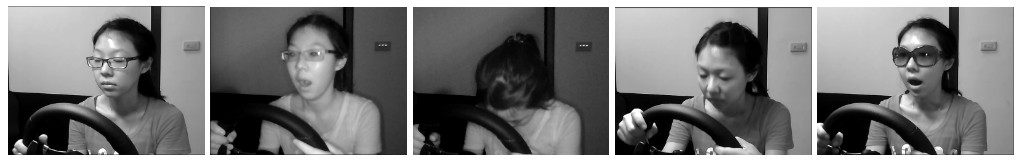
\includegraphics[width=5in]{example/NTHU2.jpg}
\caption{不同场景下的相同动作}
\label{figure:1-7}
%\end{minipage}

\end{figure}

\subsection{YawDD数据集}

\href{https://ieee-dataport.org/data-formats/video-640x480-24-bit-true-color-rgb-30-fps-avi-without-audio}{YawDD 下载地址}

\href{https://dl.acm.org/doi/10.1145/2557642.2563678}{YawDD 论文地址:YawDD: a yawning detection dataset}

YawDD数据集采集了342个视频,视频中包含不同年龄段的,不同种族的57名男性和50名女性志愿者。根据摄像头摆设位置的不同,可以细分成Dash数据集和Mirror 数据集,主要用于模拟真实驾驶环境下的哈欠检测。

\subsubsection{采集环境}

在YawDD数据集中,视频是在白天车里拍摄的,这些视频从清晨一直录制到日落。由于天气不同,晴天和雨天也会带来不同的光照情况,因此数据集在采集过程中包含各种光照条件下。在一些视频中,有一些乘客坐在辅驾驶位上,因此在视频中存在部分的背景运动。

应该注意的是,对于夜间的哈欠检测,要么必须控制车内的照明,在这种情况下,正常的白天检测方法也可以工作;要么必须使用红外摄像机来拍摄,克服图像极端黑暗的问题,但是这会导致该图像处理方法和RGB摄像机采集到的视频的处理方法完全不同。出于以上考虑,该数据集没有采集夜间视频,

\subsubsection{参与者介绍}

在YawDD数据集中,参与者坐在驾驶座上并系好安全带,以便还原真实的驾驶场景。该数据集包含57名男性和50名女性志愿者,这些志愿者来自不同的年龄、种族,具有不同的面部特征, 男女志愿者的年龄分组如图\href{figure:2-8}{2-8},图\href{figure:2-9}{2-9}所示。

在这107名志愿者中,有戴眼镜和不戴眼镜的,有留胡须和不留胡须的男人,有留胡子和不留胡子的男性,有戴围巾和不戴围巾的女性,以及有不同发型和不同衣服的人。图\href{figure:2-10}{2-10}显示了随机选择的12名志愿者。所有参与者都签署了一项协议,只允许他们的视频用于非商业和相关研究,但是只有一部分参与者同意在论文中发表他们的照片,因此对于使用该数据集并发表论文的研究人员来说,应特别注意表\href{table:2-8}{2-8}的内容,不要在论文中使用未经同意的参与者的图片。

1- Female participants:
\begin{itemize}
    \item With prescription eyeglasses : 14 people
    \item With sunglasses : 11 people
    \item Without glasses: 40 people
    \item With scarf: 3 people
    \item Without scarf: 53 people \\
\end{itemize}

2- Male participant:
\begin{itemize}
    \item With prescription eye glasses : 35 people
    \item With sunglasses : 5 people
    \item Without glasses : 33 people
    \item With moustache : 4 people
    \item Without moustache: 59 people
    \item With Beard: 7 people
    \item Without beard: 56 people
\end{itemize}

\begin{table}[!htp]

\centering
%\begin{minipage}[t]{5in}
\caption{志愿者签署协议内容(部分)}
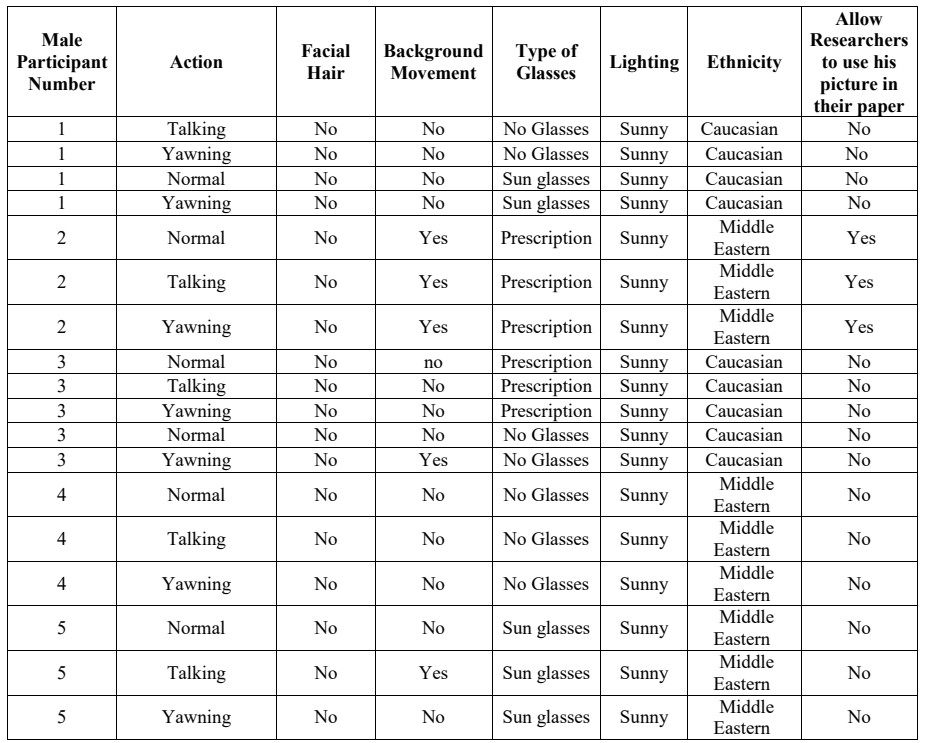
\includegraphics[width=6in]{example/researcher.jpg}
\label{table:2-8}
%\end{minipage}

\end{table}


\begin{figure}[!htp]

\centering
%\begin{minipage}[t]{5in}
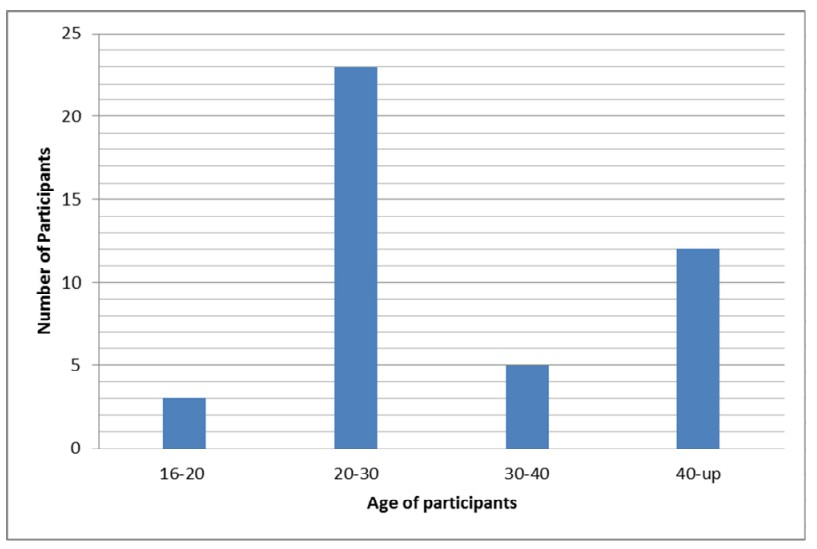
\includegraphics[width=4in]{example/female.jpg}
\caption{女性参与者年龄分组}
\label{figure:1-7}
%\end{minipage}

\end{figure}

\begin{figure}[!htp]

\centering
%\begin{minipage}[t]{5in}
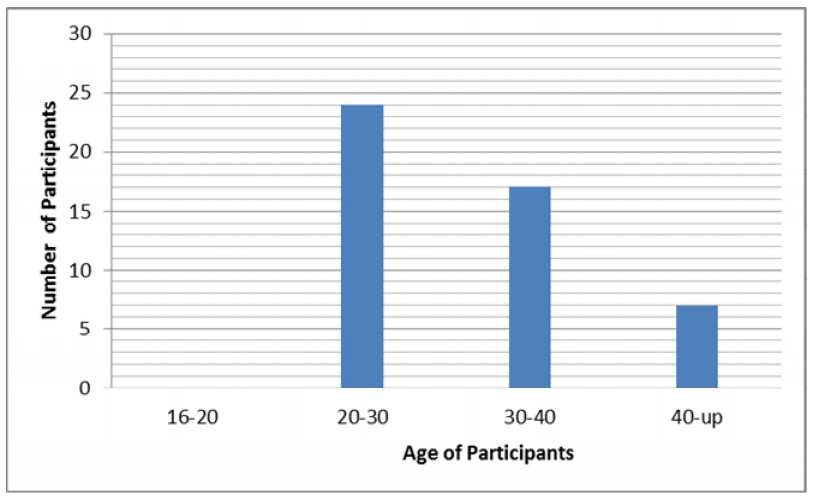
\includegraphics[width=4in]{example/male.jpg}
\caption{男性参与者年龄分组}
\label{figure:1-8}
%\end{minipage}

\end{figure}

\begin{figure}[!htp]

\centering
%\begin{minipage}[t]{5in}
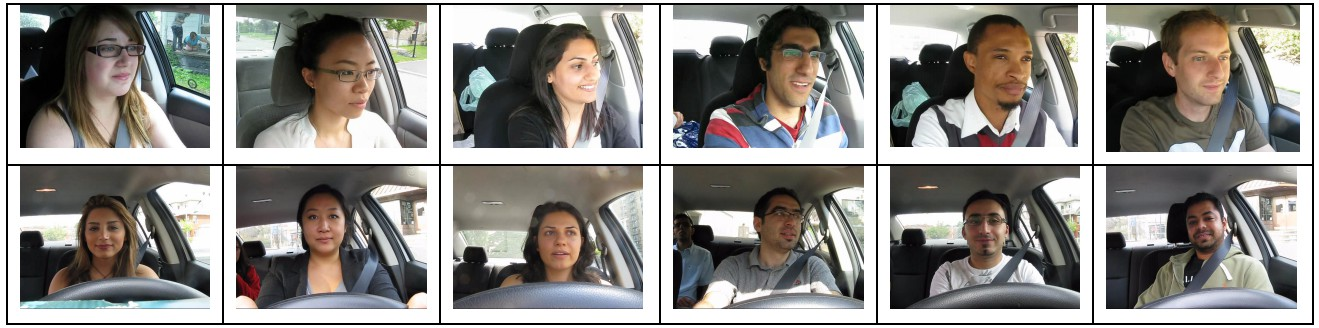
\includegraphics[width=6in]{example/dowzy.jpg}
\caption{在YawDD数据集中随机选择的12位志愿者}
\label{figure:1-8}
%\end{minipage}

\end{figure}

\subsubsection{视频介绍}

在mirror数据集(前镜摄像头)中,大多数参与者被要求拍摄三个视频。在第一视频中,参与者被要求坐在驾驶座上,系好安全带并模拟驾驶。在同一人的第二个视频中,他/她被要求在开车时说话或唱歌。第二个视频可以用来区分说话/唱歌和打哈欠,在打哈欠的情况下,这两种情况都可能使嘴巴张开,但只需检测打哈欠即可。在同一个人的第三个视频中,他/她被要求等待几秒钟,然后打个哈欠。整个视频持续时间在15-40秒之间。一些参与者被要求拍摄第四个视频,他/她们需要在谈话时打哈欠。第四个视频对研究人员来说更具挑战性,因为打哈欠正好发生在谈话过程中,因此可能更难检测到打哈欠这个动作。在有些视频中,参与者被要求佩戴太阳镜或摘下眼镜。

在dash数据集(驾驶员仪表盘上的摄像头)中,参与者被要求坐在前排座位上,并系好安全带。然后,拍摄了一段视频,参与者被要求在正常的、说话和打哈欠的姿势下开车。这三个阶段的组合有助于创建更真实的驾驶场景,同时区分这些情况并准确检测打哈欠的位置。该数据集采集了342个视频,为了压缩数据集,音频部分被删除。

\subsection{DROZY数据集}
\href{https://orbi.uliege.be/handle/2268/191620}{DROZY下载地址}

\href{http://www.drozy.ulg.ac.be/application/files/2814/5847/3536/2016Massoz.pdf}{DROZY 论文地址:The ULg Multimodality Drowsiness Database (called DROZY) and Examples of Use}

DROZY数据集中的数据来自14名年轻的健康受试者(3名男性,11名女性),随着他们保持清醒的时间的不断增加,连续进行3次长达10min的精神运动警觉测试(PVTS)。 该数据集包含多种数据格式:视频和生物电信号,而且这些数据是同步采集的。

对于每个受试者和每个PVT测试,数据集包含以下完全同步的数据:

1) KSS嗜睡量表评分:根据KSS量表,主观评估自己的困倦程度,在每个PVT开始时,KSS困倦程度从1(极度警觉)到9(非常困倦,努力保持清醒,与睡眠斗争)依次递增;

2) PVT数据:刺激时间和相应的反应时间(毫秒); 对于一个PVT,有以下三个条件
\begin{enumerate}[label=\circled{\arabic*}]
    \item 起床后3小时。
    \item 起床后21小时,并且15小时内不含咖啡因。
    \item 起床后29小时,并且15小时内不含咖啡因。
\end{enumerate}

3) 多导睡眠图(PSG)信号:5个EEG通道,2个EOG通道(水平和垂直),ECG和EMG,均以512Hz采样,并以.edf格式保存;

4) Kinect v2传感器视频:每个近红外光(NIR)辐射强度视频对应1个PVT,视频大小为512x424像素,每一帧是一个8位灰度图像,以mp4格式保存;

5) 人脸关键点(人工标注):手工选择720个视频帧(平均每个受试者51帧),并在每一帧中对68个人脸关键点进行2D(像素)和3D(毫米)标注;

6) 人脸关键点(自动标注):利用特定主题约束局部模型(CLMs)自动处理,对所有帧的68个人脸关键点进行2D和3D标注;

7) 插值指数:插值系数和最近帧的指数对于缺失帧的插值信息是必要的。

只有以下编号的受试者图片可以发表:1、2、3、6、7、8、10、11、12、13、14。如图\href{figure:2-12}{2-12} 所示。

\begin{figure}[!htp]

\centering
%\begin{minipage}[t]{5in}
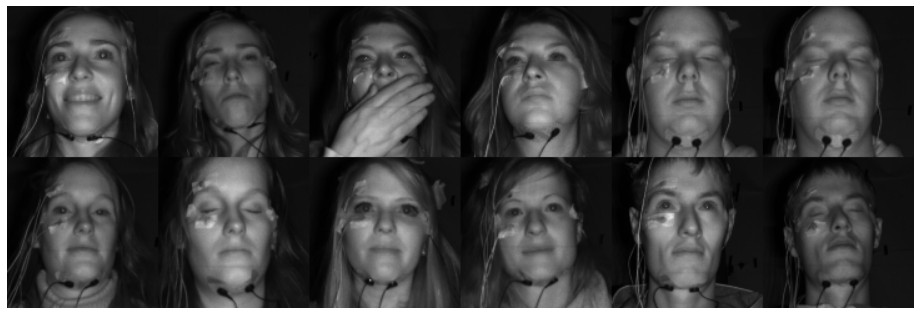
\includegraphics[width=5in]{example/drozy.jpg}
\caption{Drowzy数据集中经同意发表的11位志愿者}
\label{figure:2-12}
%\end{minipage}

\end{figure}

\section{疲劳检测模型}

图\href{2-8}{2-8}对疲劳检测模型进行了分类:生物数学模型,基于规则的模糊逻辑系统和机器学习模型。

\begin{figure}[!htp]

\centering
%\begin{minipage}[t]{5in}
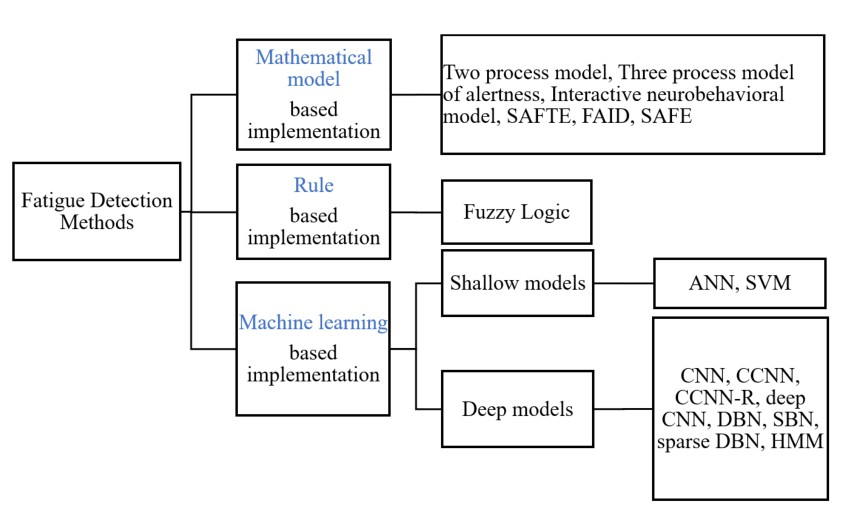
\includegraphics[width=4in]{example/model.jpg}
\caption{模型汇总}
\label{figure:1-5}
%\end{minipage}

\end{figure}

\subsection{生物数学模型}

生物数学模型利用睡眠周期这个特征对个人疲劳情况进行定量分析。生物数学模型包括的输入有:昼夜节律、睡眠时间、清醒时间和睡眠史,用来预测疲劳风险水平。两个流程模型是最早的模型之一\footnote{1982 - A two process model of sleep regulation \quad \url{https://xueshu.baidu.com/usercenter/paper/show?paperid=c141f9a4372d7d91614ad76a2df4cc5a&site=xueshu_se}}。 这个模型是基于昼夜节律过程和体内平衡过程的相互作用进行的。后来演化出了三过程模型\footnote{1995 - Validation of the S and C components of
the three-process model of alertness regulation \quad \url{https://xueshu.baidu.com/usercenter/paper/show?paperid=2da85058b9b5adb6696c3b341b9f44da&site=xueshu_se&hitarticle=1}},三过程模型利用睡眠时间和清醒时间作为输入来预测疲劳风险,并且考虑了昼夜节律和体内平衡因素。互动神经行为模型是针对那些建议调整工作时间的机构提出来的,比如航空、铁路和公共汽车运输。这个模型也是利用了体内平衡,睡眠和昼夜节律的特征\footnote{2004 - Critical research issues in development of biomathematical models of fatigue and performance \quad \url{https://xueshu.baidu.com/usercenter/paper/show?paperid=90c30e01309f9b27e4f54f60cabd4c1a&site=xueshu_se&hitarticle=1}},其中睡眠、活动、疲劳和任务效率(SAFTE) 模型是一种神经行为模型,SAFE 和SAFTE 的区别在于,SAFE是基于现实生活中生成的数据,而SAFTE是基于现实生活中的数据和自动休眠算法生成的数据。SAFTE 应用于军事、医疗和工业领域。疲劳审计InterDyne (FAID)\footnote{2004 - A model to predict work related fatigue based on hours of work \quad \url{https://xueshu.baidu.com/usercenter/paper/show?paperid=6ff16bc22412f0f35e2dfa8e7c2894b8&site=xueshu_se}} 模型仅将睡眠时间作为输入,并预测疲劳水平。FAID 模型适用于办公场所,它将疲劳程度与过去的睡眠时间联系起来。上面讨论的模型是通用模型,用于调整工作时间和提高工作效率。机组疲劳评估系统(SAFE)模型\footnote{2004 - Modeling Performance and Alertness. The QinetiQ Approach \quad \url{https://xueshu.baidu.com/usercenter/paper/show?paperid=6fe4d978bdaa008797e3bfaf70eb4e08&site=xueshu_se}} 是在实验室实验的基础上为航空旅行机组开发的,其中"SAFE"表示飞行期间的警戒级别。

大多数基于数学模型的方法都是为通用环境设计的,比如针对办公场所或者工厂里工人的工作量。近些年来,由于智能系统的发展,研究人员的注意力已经转移到智能系统,这将在下面讨论。

\subsection{模型推理系统}

基于规则的专家系统是专家系统中一种简单实现方式。对于复杂的专家系统,模糊推理系统(FIS)\footnote{2012 - Fuzzy inference
systems applied to image classification in the industrial field \quad \url{https://xueshu.baidu.com/usercenter/paper/show?paperid=a6bb4c9e7096e7781cec224aa846190e&site=xueshu_se&hitarticle=1}} 优于简单的基于规则的系统,它是以模糊集合理论和模糊推理方法等为基础,具有处理模糊信息能力的系统。模糊推理系统以模糊逻辑理论为主要计算工具,可以实现复杂的非线性映射关系,而且其输入输出都是精确的数值。当精确值进入模糊推理系统时,一般要将其模糊化成给定论域上的模糊集合。

模糊化的实质是将给定输入转换成模糊集合。模糊化的原则是:
\begin{enumerate}[label=\circled{\arabic*}]
    \item 在精确值处模糊集合的隶属度最大;
    \item 当输入有噪声干扰时,模糊化结果具有一定的抗干扰能力;
    \item 模糊化运算应尽可能简单。
\end{enumerate}

模糊推理系统设计包括:模糊化、模糊规则库、模糊推理方法及去模糊化的设计。

1)模糊规则库:模糊规则库是由模糊推理系统中的全部模糊规则组成,是模糊推理系统的核心部分。从某种意义上讲,模糊推理系统的其它部分都是为了有效地执行这些规则而存在。

2)模糊规则:
给定论域$X$和$Y$,且$x \in X$、$y \in Y$。
\begin{enumerate}[label=\circled{\arabic*}]
    \item 一维模糊规则:
        \begin{eqnarray}
            if \quad x \quad is \quad \tilde{A},\quad then \quad y \quad is \quad \tilde{B} \nonumber
        \end{eqnarray}
        其中$\tilde{A}$和$\tilde{B}$分别是论域X和Y的模糊集合。

    \item 多维模糊规则:
        \begin{align}
            & if \quad x_1 \quad is \quad \tilde{A_1} \quad and \quad x_2 \quad is \quad \tilde{A_2} \quad and \quad ... \quad and \quad x_n \quad is \quad \tilde{A_n},\quad then \quad y \quad is \quad \tilde{B} \nonumber \\
            & if \quad x_1 \quad is \quad \tilde{A_1} \quad or \quad x_2 \quad is \quad \tilde{A_2} \quad or \quad ... \quad or \quad x_n \quad is \quad \tilde{A_n},\quad then \quad y \quad is \quad \tilde{B} \nonumber
        \end{align}
        其中$\tilde{A_1},\tilde{A_2},...\tilde{A_n}$ 是论域X上的模糊集合, $\tilde{B}$是论域Y上的模糊集合。
\end{enumerate}

3)常见的模糊化方法有:模糊单值法、三角形隶属函数法、高斯隶属函数法。

4)常见的模糊推理方法有:Mamdani法、Larsen法、Zadeh法。

5)常见的去模糊化方法有:最大隶属度法、重心法、中心平均法。

FIS采用模糊规则库,并结合模糊隶属度函数进行决策。FIS 提供内置的专家知识,并使用IF-THEN基础规则将输入映射到输出。2010年,Devi和Bajaj\footnote{2010 - Fuzzy based driver fatigue detection \quad \url{https://xueshu.baidu.com/usercenter/paper/show?paperid=61f19ceaf77e3b87d90f8284a60635c2&site=xueshu_se}} 提出了一种将FIS应用于驾驶员疲劳检测的方法。将驾驶员的口、眼状态输入到FIS中,并将驾驶员的状态分为正常状态、疲劳状态和危险状态。眼睛的状态分为眨眼、困倦和睡眠,而嘴的状态则分为正常和打哈欠。

在2014年的一项研究中\footnote{2012 - Fully automated real time
fatigue detection of drivers through fuzzy expert systems \quad \url{https://xueshu.baidu.com/usercenter/paper/show?paperid=8044564aebf163ea4ddab21d9b6784d8&site=xueshu_se}},作者将眼睛状态和嘴状态特征输入到两层的FIS 系统中,来预测驾驶员的疲劳程度。FIS的每一层都有自己的IF-THEN规则,可以从特定的输入推导输出。FIS 提供了高度的灵活性,在许多基于视觉的应用程序中非常有用。FIS提供较少数据的训练,并在所有规则同时应用时提供并行处理。FIS还具有通过整合额外规则和知识库进行学习的能力。



\subsection{机器学习模型}
机器学习算法需要通过从实验室或者道路测试中获取到的大量驾驶数据来训练模型。根据表征水平的不同,这类模型可以分为浅层模型和深度学习模型。

\subsubsection{浅层模型}

浅层模型相较于深度学习模型,具有较低的计算复杂度,并具有预测功能。浅层模型不需要大量的训练数据,但需要从数据中预先定义具有区分性的特征。众所周知,包含一个隐藏层的人工神经网络(ANN)和支持向量机(SVM),都是浅层模型。

ANN通过模仿人类大脑来处理信息,其中,ANN包括监督、非监督或强化学习模式。神经网络已经广泛应用于疲劳检测系统\footnote{Applying neural
network analysis on heart rate variability data to assess driver fatigue \quad \url{https://xueshu.baidu.com/usercenter/paper/show?paperid=3cb5c7d63a7afbb59cbd6adcd1ff7006&site=xueshu_se}},神经网络可以根据各种数据进行模型的训练,比如脑电图(EGG)、 转向角度(SWA)和PERCLOS来预测驾驶员疲劳或警觉状态。在2002 年《\href{https://xueshu.baidu.com/usercenter/paper/show?paperid=283463e03da84178acd0dca1591bb0ea&site=xueshu_se&hitarticle=1}{Automatic
recognition of alertness and drowsiness from EEG by an artificial neural network}》一文中,作者从脑电信号(EGG) 的时间序列中,提取左右脑间和脑内的交叉谱密度,将其输入到神经网络中,其中驾驶员疲劳状态分为两类:疲劳和警觉。在2006年《\href{https://xueshu.baidu.com/usercenter/paper/show?paperid=8b2148521959fcd0f7678e4f703e4b76&site=xueshu_se}{Early Driver Fatigue Detection from Electroencephalography Signals using Artificial Neural Networks}》一文中,作者提出了另一种方法:将脑电时域信号转换为频域信号,得到$\alpha$、$\theta$、$\beta$ 和$\theta$频带,并将频域数据送入神经网络进行疲劳检测。Friedrichs和Yang在《\href{https://xueshu.baidu.com/usercenter/paper/show?paperid=2b397a7cad2d13149573e400b0a83398&site=xueshu_se&hitarticle=1}{Drowsiness monitoring by steering and lane
data based features under real driving conditions}》一文中,同时将基于车道的特征和基于转向的特征输入到神经网络中,并将驾驶员驾驶状态为三类:清醒、疲劳和可疑。

支持向量机(SVM)是专门为二分类问题设计的,支持向量机已经应用于许多疲劳检测系统中,根据不同的疲劳程度对驾驶员的状态进行分类。SVM可以根据EEG、ECG、PERCLOS、EoG 等参数,对疲劳状态进行分类。Mervyn等\footnote{Can SVM be used for automatic EEG detection of drowsiness during car driving? \quad \url{https://xueshu.baidu.com/usercenter/paper/show?paperid=832535a2c8f5fce7435383dd05e0eb83&site=xueshu_se}} 通过训练SVM,对两类疲劳进行分。他们发现,人处于警觉状态时,$\beta$波明显,当人开始处于疲劳状态时,$\alpha$波有明显下降趋势。该方法的分类准确率可以达到99.2$\%$。另外,有些研究者\footnote{Detection of driver drowsiness using wavelet analysis of heart rate variability and a support vector machine classifier \quad \url{https://xueshu.baidu.com/usercenter/paper/show?paperid=ff6ce7a5353e5830f88f2ef24de4a947&site=xueshu_se}} 通过从光容积描记术(PPG) 中提取的心血管血容量、脉搏和心率变异性(HRV) 等特征来训练支持向量机。 对HRV数据进行快速傅里叶变换(FFT) 和小波分解。提取低频(LF)高频(HF),对小波分解得到的数据进行特征的选择,然后将LF,HF和特征选择得到的特征输入到SVM中,对驾驶员的状态分类(警报或疲劳)。

\subsubsection{深度学习模型}

深度学习模型是一种数据特征自动化提取技术,而不是关于特定任务的方法,与浅层模型相比,深层模型具有从训练数据中提取特征的能力。卷积神经网络(CNN) 是最早用于驾驶员疲劳检测的深度学习模型。在2014年《\href{https://xueshu.baidu.com/usercenter/paper/show?paperid=a9b574549a36e94db6af2b728361eee9&site=xueshu_se&hitarticle=1}{Drowsy driver detection
using representation learning}》一文中,作者利用CNN学习到的特征,通过一个softmax层将驾驶员状态分为嗜睡状态或非嗜睡状态。使用Viola-Jones方法从帧中提取人脸,并输送给CNN进行特征提取,softmax层根据提取的特征进行训练。在实验中,20$\%$的数据被用于测试。对于驾驶员的疲劳检测,信道级卷积神经网络(CCNN)和CCNN-R显示出比CNN更好的效果\footnote{Prediction of driver's drowsy and alert states from EEG signals with deep learning \quad \url{https://xueshu.baidu.com/usercenter/paper/show?paperid=a5d49d89b38c74777da8d2a6d4562791&site=xueshu_se&hitarticle=1}}。CCNN-R 使用受限的玻尔兹曼机代替卷积核进行特征提取,并使用bagging 分类器对驾驶员疲劳状态进行分类。打哈欠是疲劳的一个显著特征,大量的研究通过利用哈欠检测来检测疲劳驾驶状态。在《\href{https://xueshu.baidu.com/usercenter/paper/show?paperid=1e648bec62633991942caf1104f4efbb&site=xueshu_se&hitarticle=1}{Driver yawning detection based on deep convolutional neural learning and robust nose tracking}》一文中,作者使用两个深度CNN模型,一个用于人脸检测,另一个用于鼻子检测。由于鼻子具有明显的跟踪特征,因此相比于嘴巴跟踪,人们更喜欢对鼻子跟踪进行研究,而且从鼻子的位置我们可以推断出嘴的位置。

深度信念网络(DBN)是另一种深度学习模型,它由多层隐藏单元组成。层之间是相互连接的,但是单个层中的单元是不连接的。2017年,Chai等\footnote{Improving EEG-based driver fatigue classification using sparse-deep belief networks \quad \url{https://xueshu.baidu.com/usercenter/paper/show?paperid=ce1a8c4e000831289e28253b7ecf55ea&site=xueshu_se&hitarticle=1}} 研究了稀疏DBN在基于EEG的疲劳检测中的有效性。稀疏DBN是一种半监督学习方法,用于预训练层的特征建模和下一层的特征识别。实验结果表明稀疏DBN分类器的疲劳检测精度高于神经网络分类器以及DBN分类器。

贝叶斯网络是一种概率图模型,它可以根据训练数据或专家意见建立。静态贝叶斯网络(SBN)可用来预测疲劳\footnote{2004 - Real-time nonintrusive monitoring and
prediction of driver fatigue \quad \url{https://xueshu.baidu.com/usercenter/paper/show?paperid=1b904eacc029951ebb44b2d7a2bbc0fb&site=xueshu_se}},然而,SBN对于随时间变化的系统适用性相对较差。为了解决这一问题,考虑动态贝叶斯网络(DBN)\footnote{2005 - Active affective State detection and user assistance
with dynamic Bayesian networks \quad \url{https://xueshu.baidu.com/usercenter/paper/show?paperid=dfb3c369e3f830842f3eafa9a4b2d288&site=xueshu_se}} 进行驾驶员疲劳检测,动态建模驾驶员状态。在2006年《\href{https://xueshu.baidu.com/usercenter/paper/show?paperid=6169446ab4e1e341d4e8b342f349b874&site=xueshu_se}{A probabilistic framework for modeling and real-time monitoring human fatigue}》一文中,作者提出的动态贝叶斯模型并没有考虑到生理特征,而是依赖于视觉特征进行疲劳检测。而在2010年的《\href{https://xueshu.baidu.com/usercenter/paper/show?paperid=77b329aa91601b793fd7bd3d22cbefa8&site=xueshu_se&hitarticle=1}{A driver fatigue recognition
model based on information fusion and dynamic Bayesian network}》一文中,Yang 等提出了一种基于视觉和生理特征的DBN模型。

最简单的DBN可以用隐马尔可夫模型(HMM)来建模。HMM是一种基于隐马尔科夫过程的统计模型,在已知状态转移概率情况下,该模型存在两种状态之间的移动。为了通过当前和之前的状态预测驾驶员未来的状态,2016年作者在《\href{https://xueshu.baidu.com/usercenter/paper/show?paperid=fbdc243ba7aa1adf749a692d9536fb44&site=xueshu_se}{Dynamic driver fatigue detection using
hidden Markov model in real driving condition}》一文中使用了一阶HMM模型,并利用睡眠史、驾驶情况和昼夜节律特征来疲劳预测。

\section{疲劳检测难点}

1、基于计算机视觉的人脸疲劳检测所面临的难点\footnote{\url{https://www.sohu.com/a/238118192_100163862}}

1)光照问题

光照变化是影响人脸识别性能的最关键因素,对该问题的解决程度关系着人脸识别实用化进程的成败。由于人脸的3D结构,光照投射出的阴影,会加强或减弱原有的人脸特征。尤其是在夜晚,由于光线不足造成的面部阴影会导致识别率的急剧下降,使得系统难以满足实用要求。

2)姿态问题

人脸识别主要依据人的面部表象特征来进行,如何识别由姿态引起的面部变化就成了该技术的难点之一。姿态问题涉及头部在三维垂直坐标系中绕三个轴的旋转造成的面部变化,其中垂直于图像平面的两个方向的深度旋转会造成面部信息的部分缺失。使得姿态问题成为人脸识别的一个技术难题。针对姿态的研究相对比较的少,目前多数的人脸识别算法主要针列正面、准正面人脸图像,当发生俯仰或者左右侧而比较厉害的情况下,人脸识别算法的识别率也将会急剧下降。

3)表情问题

面部幅度较大的哭、笑、愤怒等表情变化同样影像着面部识别的准确率。现有的技术对这些方面处理得还不错,论是张嘴还是做一些夸张的表情,计算机都可以通过三维建模和姿态表情校正的方法把它纠正出来。

4)遮挡问题

对于非配合情况下的人脸图像采集,遮挡问题是一个非常严重的问题。特别是在监控环境下,往往被监控对象都会带着眼镜、帽子等饰物,使得被采集出来的人脸图像有可能不完整,从而影响了后面的特征提取与识别,甚至会导致人脸检测算法的失效。

5)年龄变化

随着年龄的变化,一个人从少年变成青年,变成老年,他的容貌可能会发生比较大的变化,从而导致识别率的下降。对于不同的年龄段,人脸识别算法的识别率也不同。这个问题最直接的例子就是身份证照片的识别,在我国身份证的有效期一般都是20 年,这20年间每个人的容貌必然会发生相当大的变化,所有在识别上也同样存在很大的问题。

2、个体行为差异对疲劳检测的影响

在预定时间点的疲劳症状被认为是当前时间点疲劳的一个因素,但是根据个体行为变化的不同,时间点也可能会发生变化。例如,打哈欠是疲劳的主要症状,但它并不总发生在司机睡觉前。因此在疲劳检测种中,对于单个时间点的疲劳检测应该作为一个初步阶段,并且在这一步中应该包含对驾驶员眼睛状况的评估。

